%        File: arfc-beamer.tex
%     Created: Sun May 5 10:00 PM 2013 C
%


%\documentclass[11pt,handout]{beamer}
\documentclass[9pt]{beamer}
\usetheme[white]{Illinois}
%\title[short title]{long title}
\title[Spent Fuel]{International Spent Nuclear Fuel Options}

%\subtitle[short subtitle]{long subtitle}
\subtitle[ENG 471]{ENG 471 Seminar}
%\author[short name]{long name}
\author[K. Huff]{Kathryn Huff\\Advanced Reactors and Fuel Cycles 
Group\\\url{http://katyhuff.github.io/2017-09-27-ne471.pdf}}
%\date[short date]{long date}
\date[09.27.2017]{September 27, 2017}
%\institution[short name]{long name}
\institute[UIUC]{University of Illinois at Urbana-Champaign}

%\usepackage{bbding}
\usepackage{amsfonts}
\usepackage{amsmath}
\usepackage{xspace}
\usepackage{graphicx}
\usepackage{subfigure}
\usepackage{booktabs} % nice rules for tables
\usepackage{microtype} % if using PDF
\usepackage{bigints}
\usepackage{minted}

\newcommand{\units}[1] {\:\text{#1}}%
\newcommand{\SN}{S$_N$}%{S$_\text{N}$}%{$S_N$}%
\DeclareMathOperator{\erf}{erf}
%I need some complimentary error funcitons... 
\DeclareMathOperator{\erfc}{erfc}
%page numbers
\setbeamertemplate{footline}[page number]
\setbeamertemplate{caption}[numbered]
%Those icons in the references are terrible looking
\setbeamertemplate{bibliography item}[text]

%%%% Acronym support

\usepackage[acronym,toc]{glossaries}
\include{acros}

\makeglossaries

%try to get rid of header on title page\dots
\makeatletter
    \newenvironment{withoutheadline}{
        \setbeamertemplate{headline}[default]
        \def\beamer@entrycode{\vspace*{-\headheight}}
    }{}
\makeatother

\usepackage{draftwatermark}
\begin{document}
%%%%%%%%%%%%%%%%%%%%%%%%%%%%%%%%%%%%%%%%%%%%%%%%%%%%%%%%%%%%%
%% From uw-beamer Here's a handy bit of code to place at 
%% the beginning of your presentation (after \begin{document}):
\newcommand*{\alphabet}{ABCDEFGHIJKLMNOPQRSTUVWXYZabcdefghijklmnopqrstuvwxyz}
\newlength{\highlightheight}
\newlength{\highlightdepth}
\newlength{\highlightmargin}
\setlength{\highlightmargin}{2pt}
\settoheight{\highlightheight}{\alphabet}
\settodepth{\highlightdepth}{\alphabet}
\addtolength{\highlightheight}{\highlightmargin}
\addtolength{\highlightdepth}{\highlightmargin}
\addtolength{\highlightheight}{\highlightdepth}
\newcommand*{\Highlight}{\rlap{\textcolor{HighlightBackground}{\rule[-\highlightdepth]{\linewidth}{\highlightheight}}}}
\setcounter{tocdepth}{2}
%%%%%%%%%%%%%%%%%%%%%%%%%%%%%%%%%%%%%%%%%%%%%%%%%%%%%%%%%%%%%
%%--------------------------------%%
\begin{withoutheadline}
\frame{
  \titlepage
}
\end{withoutheadline}

%%--------------------------------%%
\AtBeginSection[]{
\begin{frame}
  \frametitle{Outline}
  \tableofcontents[currentsection]
\end{frame}
}

\begin{frame}
  \frametitle{Interactive Slides}
  {\Large
  The web-interactive first half of the talk can be found at:\\

  {\color{orange}\url{https://katyhuff.github.io/2017-09-27-eng471}}}
\end{frame}

\section{Introduction}
\subsection{Nuclear Nations}

\begin{frame}
  \frametitle{Nuclear Power Nations}
  % a comment
  \begin{figure}[htbp!]
    \begin{center}
      \includegraphics[width=\textwidth]{./images/nuclear-nations-map.png}\\

\vspace{-10mm}
      \includegraphics[height=0.2\textheight]{./images/nuclear-nations-legend.png}
    \end{center}
          \caption{Nuclear power status of all nations 
          \cite{paleogene_file:nuclear_2017}.}
    \label{fig:nuc-nations-map}
  \end{figure}
\end{frame}

\begin{frame}
  \frametitle{Nuclear Weapons Nations}
  % a comment
  \begin{figure}[htbp!]
    \begin{center}
      \includegraphics[width=\textwidth]{./images/nuclear-weapons-map.png}\\

\vspace{-10mm}
      \includegraphics[height=0.2\textheight]{./images/nuclear-weapons-legend.png}
    \end{center}
          \caption{Nuclear weapons status of all nations 
          \cite{paleogene_file:nuclear_2017}.}
    \label{fig:nuc-nations-map}
  \end{figure}
\end{frame}




\begin{frame}
  \frametitle{Power vs. Weapons}
  % a comment
        \begin{columns}
                \column[t]{0.6\textwidth}
        \begin{center}
      \includegraphics[width=\textwidth]{./images/nuclear-nations-map.png}\\
    \end{center}
                \column[t]{0.6\textwidth}
\hspace{-1in}
                \begin{center}
		      \includegraphics[width=\textwidth]{./images/nuclear-weapons-map.png}
                \end{center}
        \end{columns}
\end{frame}        

\begin{frame}
  \frametitle{International Reactors}
  % a comment
  \begin{figure}[htbp!]
    \begin{center}
      \includegraphics[width=\textwidth]{./images/nuclear-nations.eps}
    \end{center}
          \caption{Nuclear reactors internationally, replicated from 
          \cite{iaea_country_2015}.}
    \label{fig:nuc-nations}
  \end{figure}
\end{frame}

\begin{frame}
  \frametitle{Nuclear Capacity}
  \begin{figure}[htbp!]
    \begin{center}
      \includegraphics[width=0.9\textwidth]{./images/nuclear-nations-deployments.png}
    \end{center}
          \caption{Nuclear power deployments as a function of time
          \cite{torsch_global_2013}.}
    \label{fig:nuc-nations-deployments}
\end{figure}
\end{frame}


\subsection{Spent Fuel Inventory}


\begin{frame}[fragile]
        \frametitle{Spent Fuel Inventory}
    \begin{table}
      \centering
      \begin{tabular}{l|lll}
        \multicolumn{4}{c}{\textbf{Radioactive Waste Volumes}}\\
        \hline
Type & In storage ($m^3$) & In disposal ($m^3$)  &  \% in disposal\\
        \hline
VLLW &   2,356,000 &   7,906,000  &  77\%\\
LLW  &  3,479,000  &  20,451,000 &   85\%\\
ILW  &  460,000  &  107,000  &  19\%\\
HLW  &  22,000 &   0   & 0\%\\
        \hline
      \end{tabular}
      \caption[SNF volumes]{Solid radioactive waste volumes worldwide, IAEA 
      estimate 2016. \cite{iaea}}
      \label{tab:vol}
    \end{table}
    \end{frame}

\begin{frame}[fragile]
        \frametitle{VLLW, LLW, ILW}
        \begin{block}{Liquid}
                Must be solidified or, must be packed in absorbant package 2x liquid volume.
                (i.e. decontamination solutions, liquid scintillators, 
                ion-exchange fluids, etc.)
        \end{block}
        \begin{block}{Wet Solid}
                Greater than 1\% liquid, but primarily solid (i.e. filters).
        \end{block}
        \begin{block}{Dry Solid}
                        Less than 1\% liquid (i.e. trash, swipes, clothes, 
                        tools, etc.)
        \end{block}
\end{frame}

\begin{frame}[fragile]
        \frametitle{Spent Fuel Inventory}
                \begin{figure}[htb!]
  \begin{center}
    \includegraphics[height=0.7\textheight]{./images/fuel_assembly.eps}
  \end{center}
  \caption{Spent nuclear fuel from conventional power reactors is in the form of 
    uranium oxide fuel rods \cite{nrc_nuclear-fuel.jpg_????}.}
  \label{fig:snf}
\end{figure}

\end{frame}

\begin{frame}[fragile]
        \frametitle{Spent Fuel}
        \begin{figure}
        \includegraphics[width=\textwidth]{./images/ewing-microstructure}
                \caption{Microstructure of spent fuel and the distribution of 
                fission products and actinides after irradiation in a reactor. 
                From \cite{ewing_long-term_2016}.}
        \end{figure}
\end{frame}

\begin{frame}[fragile]
        \frametitle{Spent Fuel Inventory}
\begin{block}{High Level Waste}
        \begin{itemize}
                \item 300,000 metric tons worldwide 
                        \cite{ewing_long-term_2016} 
                \item 90\% in storage pools 
                \item remainder in dry casks
        \end{itemize}
        \end{block}
\end{frame}


\section{Spent Fuel Options}

%%--------------------------------%%
\begin{frame}[c]
    \frametitle{Array of Possible Options}
    \begin{figure}[htbp!]
  \begin{center}
    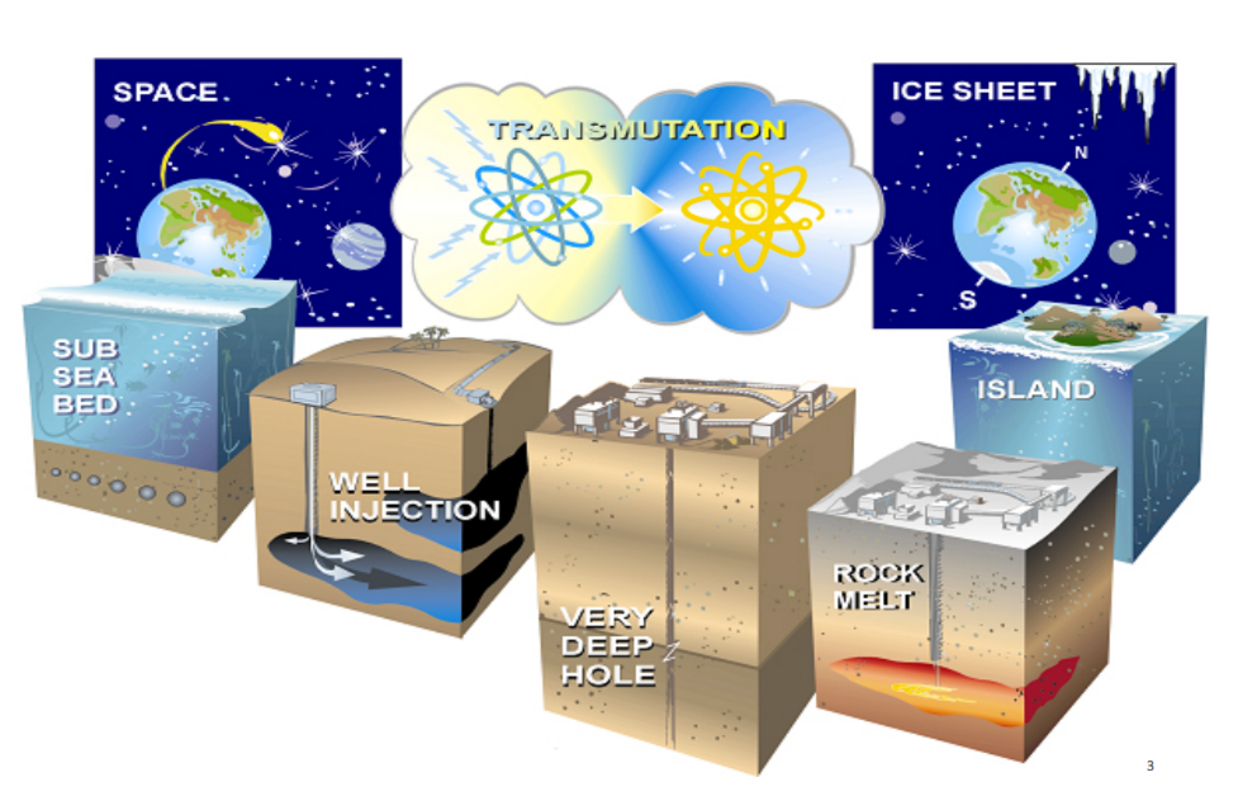
\includegraphics[height=0.7\textheight]{./images/alternative_options.eps}
  \end{center}
  \caption{An array of options have been considered in the past 
    \cite{peters_whats_2013}.}
  \label{fig:alternative_options}
\end{figure}

  \end{frame}

\subsection{Long-Term Storage}

\begin{frame}[fragile]
        \frametitle{VLLW, LLW, ILW}
                

  \begin{figure}[htbp!]
    \begin{center}
    \begin{minipage}[t]{0.44\textwidth}
      \includegraphics[width=\textwidth]{./images/llw-disposal-cartoon}
      \caption{Design of a LLW repository.}
        \label{fig:llw-cartoon}
    \end{minipage}
    \hspace{0.01\textwidth}
    \begin{minipage}[t]{0.44\textwidth}
      \includegraphics[width=\textwidth]{./images/wcs-andrews-tx.png}
      \caption{Waste Control Specialists Low Level Waste Repository in Andrews 
            County, Tx.}
        \label{fig:wcs}
    \end{minipage}
    \end{center}
  \end{figure}



\end{frame}

\begin{frame}[fragile]
        \frametitle{Spent Fuel Inventory}
                

  \begin{figure}[htbp!]
    \begin{center}
    \begin{minipage}[t]{0.45\textwidth}
      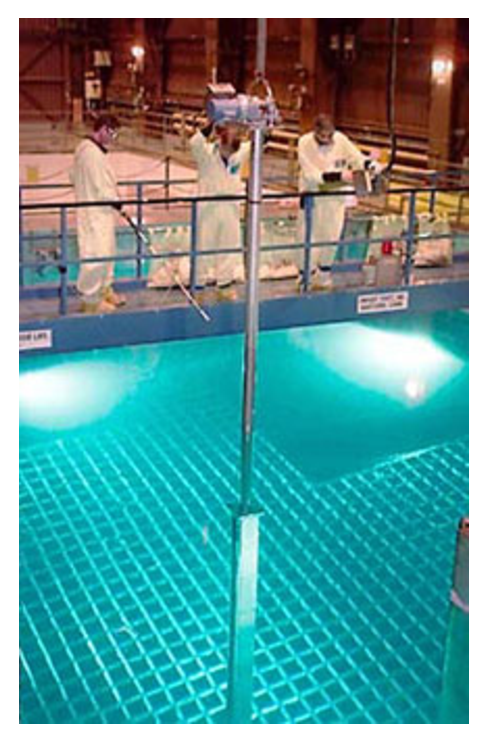
\includegraphics[height=0.4\textheight]{./images/pool.eps}
      \caption{Spent fuel pools are at reactor sites and elsewhere 
        \cite{doe_spent_????}.}
        \label{fig:pool}
    \end{minipage}
    \hspace{0.01\textwidth}
    \begin{minipage}[t]{0.45\textwidth}
      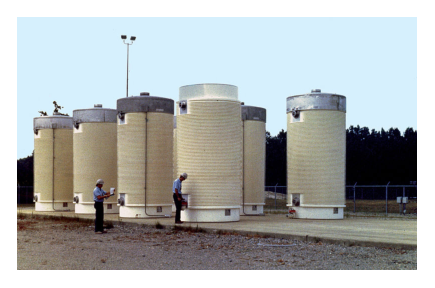
\includegraphics[height=0.4\textheight]{./images/casks.eps}
      \caption{Dry casks at reactor sites and elsewhere \cite{nrc_dry_2008}}
        \label{fig:casks}
    \end{minipage}
    \end{center}
  \end{figure}

\end{frame}


\begin{frame}[fragile]
        \frametitle{Reprocessing Waste}
                \begin{figure}[htbp!]
  \begin{center}
    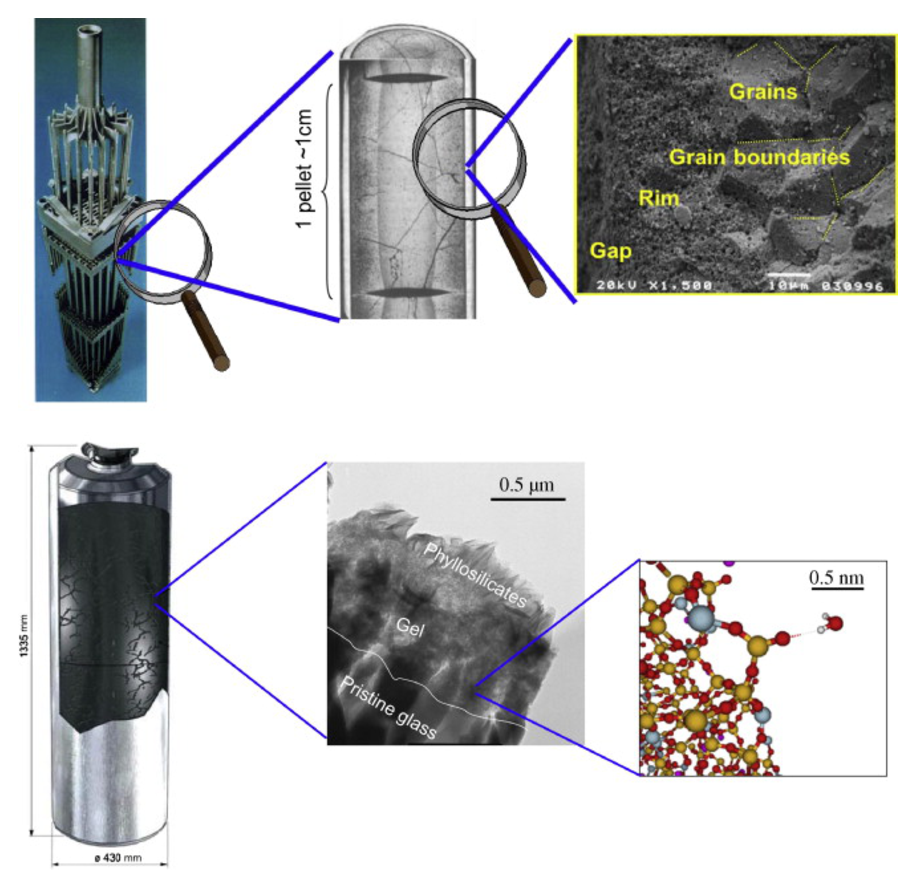
\includegraphics[width=0.5\textwidth]{./images/waste_forms_poinssot.eps}
  \end{center}
  \caption{A comparison of uranium oxide and borosilicate glass waste forms 
  \cite{poinssot_long-term_2012}.}
  \label{fig:waste_forms_poinssot}
\end{figure}

\end{frame}

\begin{frame}[fragile]
        \frametitle{Reprocessing Waste}
                

  \begin{figure}[htbp!]
    \begin{center}
    \begin{minipage}[t]{0.45\textwidth}
      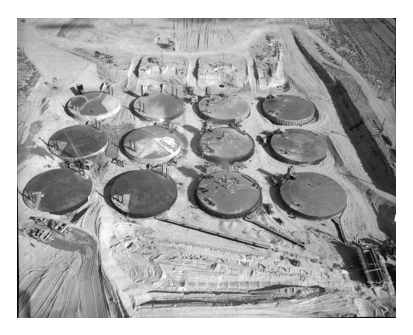
\includegraphics[height=0.4\textheight]{./images/tanks.eps}
        \caption{Liquid waste in steel or carbon steel tanks at Hanford and 
          elsewhere\cite{doe_underground_????}.}
        \label{fig:tanks}
    \end{minipage}
    \hspace{0.01\textwidth}
    \begin{minipage}[t]{0.45\textwidth}
      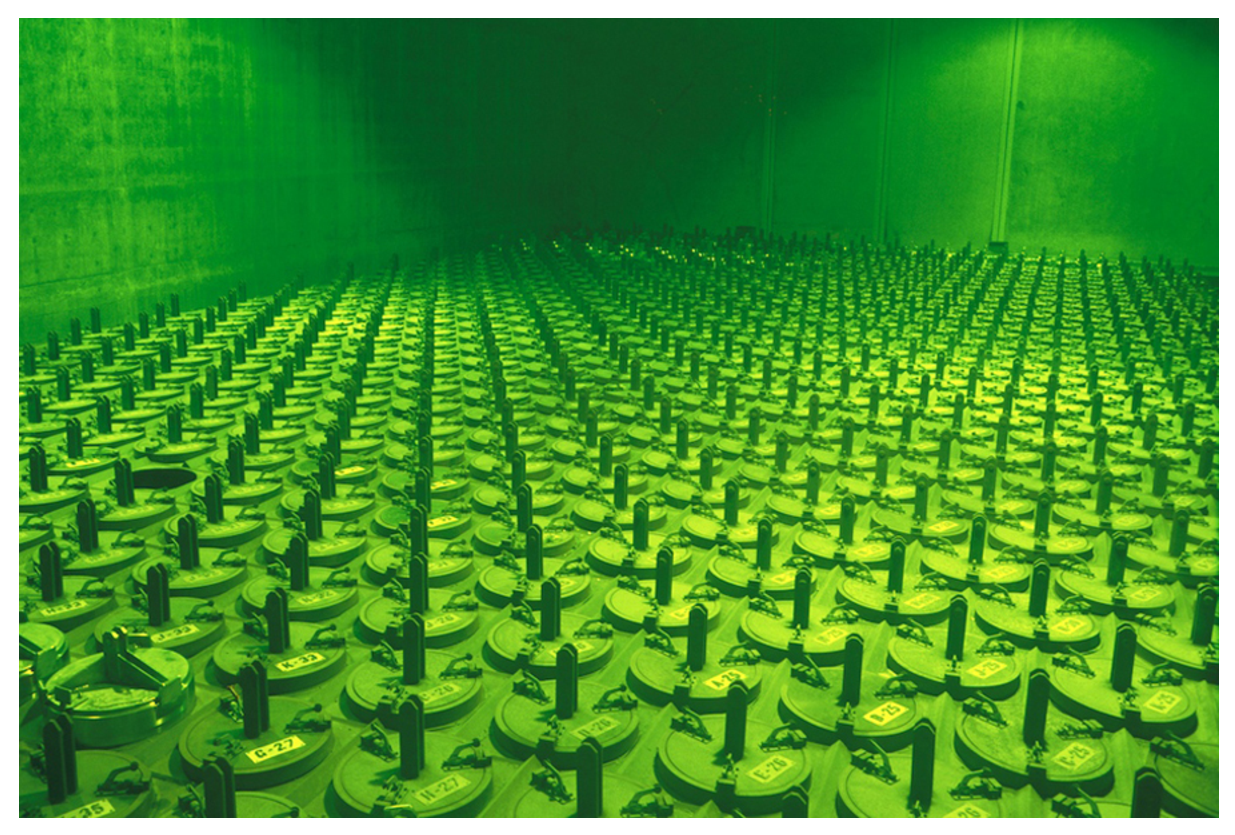
\includegraphics[height=0.4\textheight]{./images/logs.eps}
        \caption{Vitrified glass logs at reprocessing facilities and elsewhere 
          \cite{essick_photographing_2012}.}
        \label{fig:logs}
    \end{minipage}
    \end{center}
  \end{figure}

\end{frame}


\subsection{Reprocessing}

\begin{frame}
  \frametitle{Reprocessing Capacity}
  % a comment
  Global reprocessing capacity is shown in Fig. \ref{fig:reprocessing-nn}.
  \begin{figure}[htbp!]
    \begin{center}
      \includegraphics[width=\textwidth]{./images/reprocessing-nn}
    \end{center}
          \caption{\cite{buckner_case_2016}.}
    \label{fig:reprocessing-nn}
  \end{figure}
\end{frame}

\begin{frame}
  \frametitle{MOX production}
  % a comment
  Global MOX production is shown in Fig.
  \ref{fig:mox-production-nn}.
  \begin{figure}[htbp!]
    \begin{center}
      \includegraphics[height=4cm]{./images/mox-production-nn}
    \end{center}
          \caption{\cite{buckner_case_2016}.}
    \label{fig:mox-production-nn}
  \end{figure}
\end{frame}

\subsection{Deep Geologic Disposal}
% layouts
% EBS choices
% Geologies


\begin{frame}[c]
  \frametitle{Clay Disposal Environments}

  \begin{figure}[h!]
    \begin{center}
      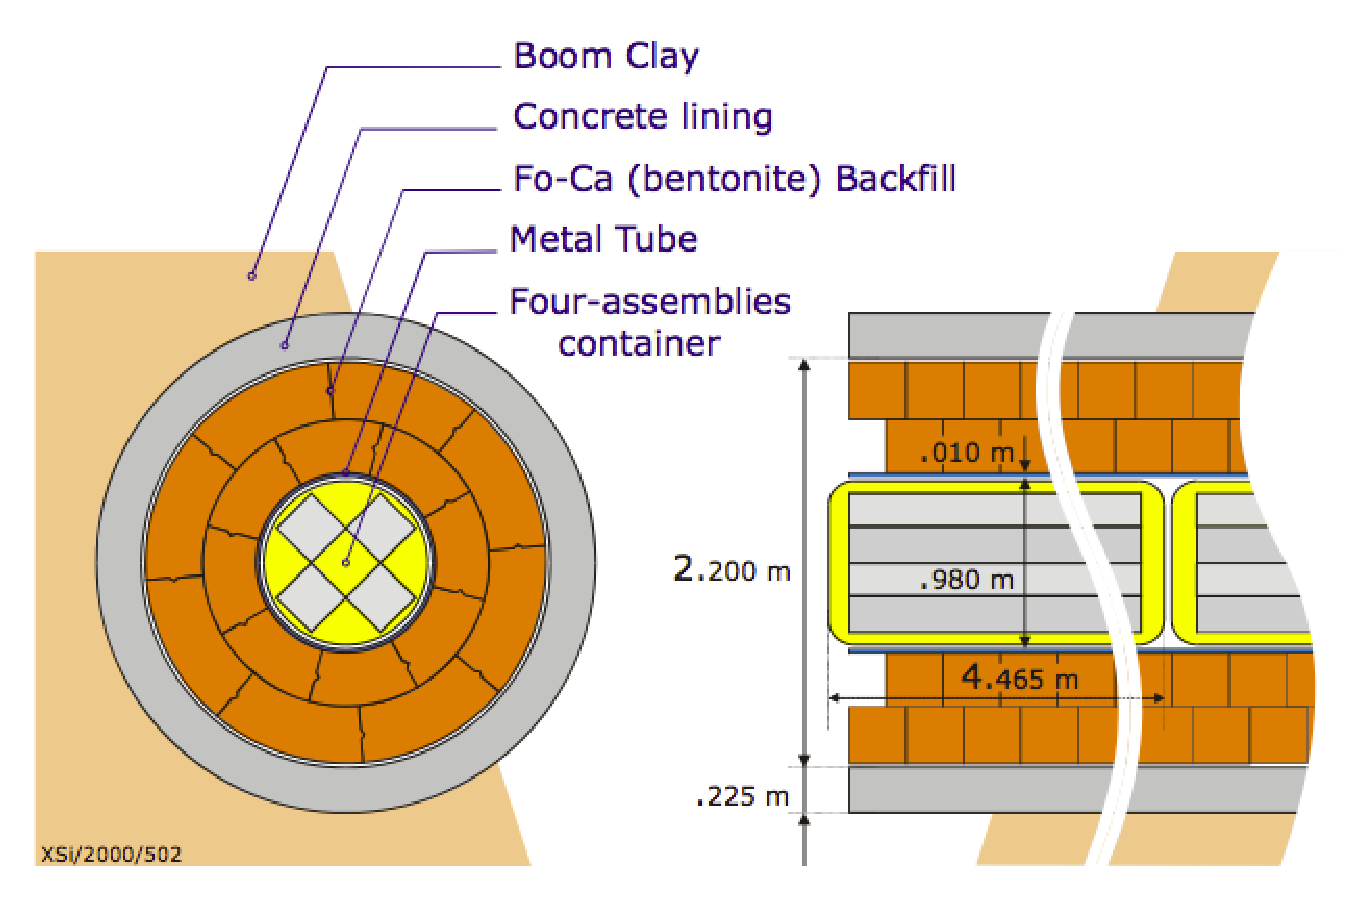
\includegraphics[height=.7\textheight]{./images/belgianClayRedImp.eps}
    \end{center}
    \caption{Belgian reference concept in Boom Clay 
    \cite{von_lensa_red-impact_2008}.}
    \label{fig:belgianClayRedImp}
  \end{figure}

\end{frame}

\begin{frame}[c]
  \frametitle{Granite Disposal Environments}

  \begin{figure}[h!]
    \begin{center}
      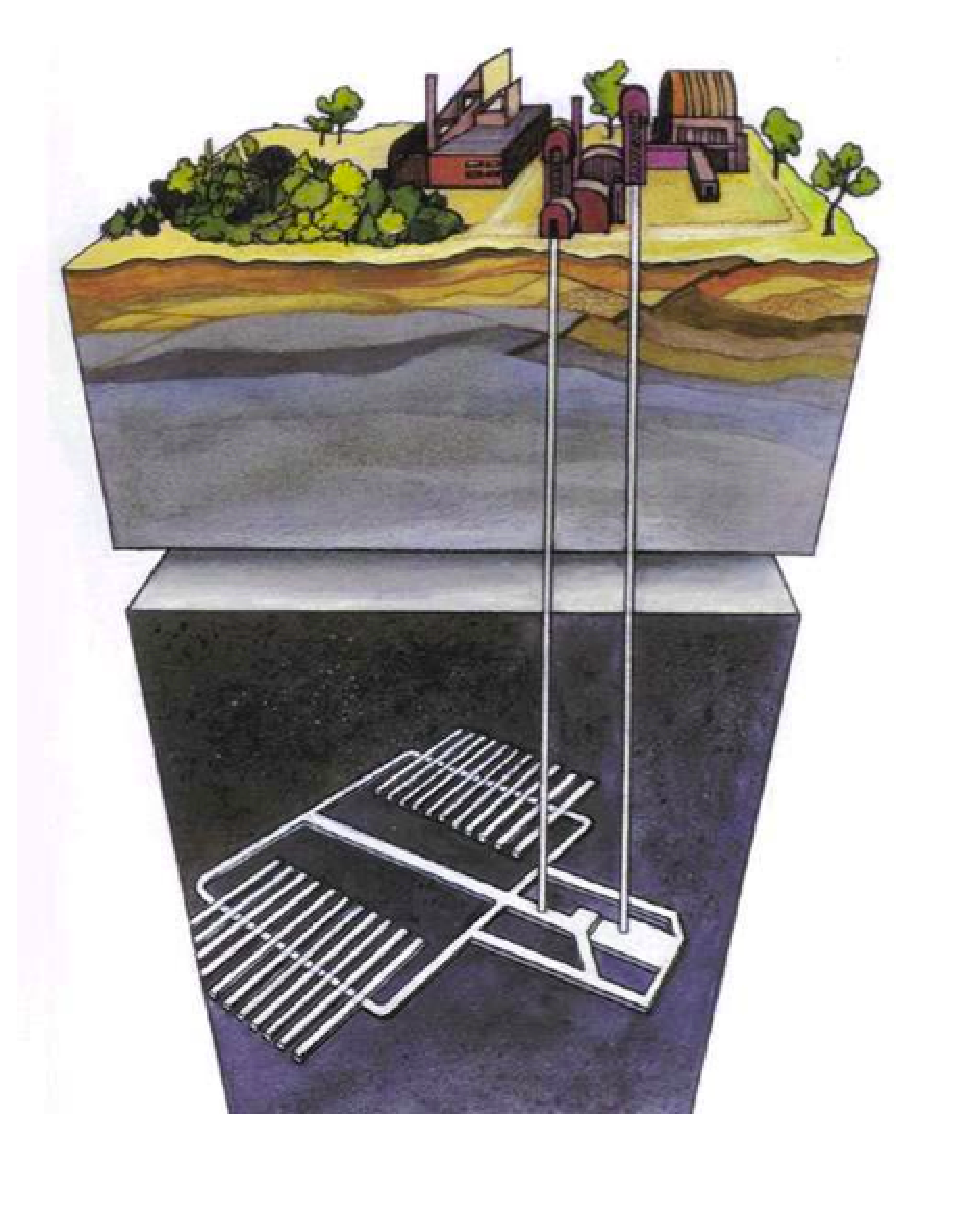
\includegraphics[height=.7\textheight]{./images/czechGraniteRedImp.eps}
    \end{center}
    \caption{Czech reference concept in Granite 
    \cite{von_lensa_red-impact_2008}.}
    \label{fig:czechGraniteRedImp}
  \end{figure}

\end{frame}

\begin{frame}[c]
  \frametitle{Salt Disposal Environments}

  \begin{figure}[h!]
    \begin{center}
      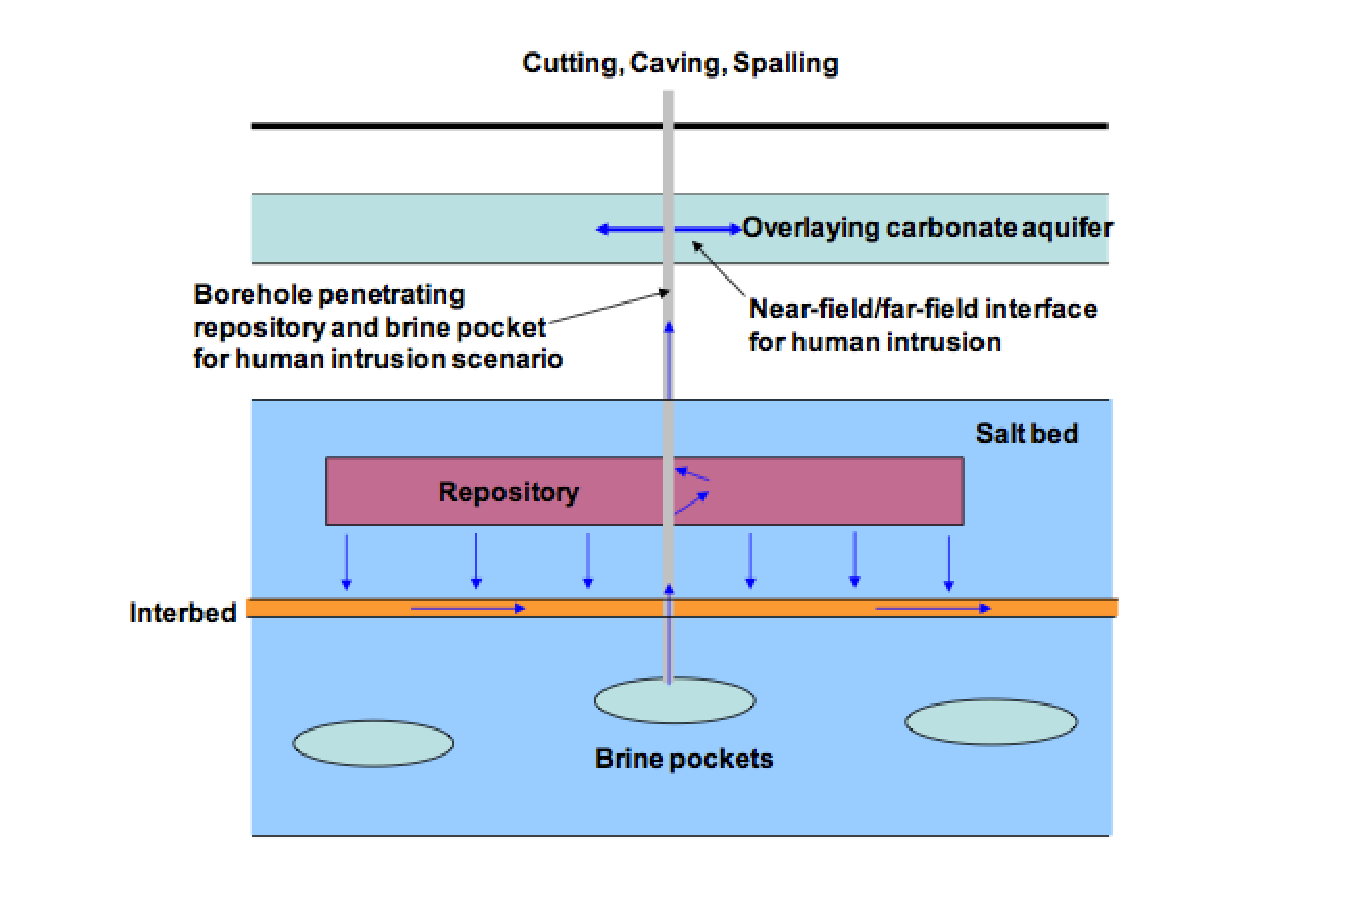
\includegraphics[height=.7\textheight]{./images/saltGPAM.eps}
    \end{center}
    \caption{DOE-NE Used Fuel Disposition Campaign  concept in 
    Salt \cite{clayton_generic_2011}.}
    \label{fig:saltGPAM}
  \end{figure}

\end{frame}

\begin{frame}[c]
  \frametitle{Deep Borehole Disposal Environment}

  \begin{figure}[h!]
    \begin{center}
      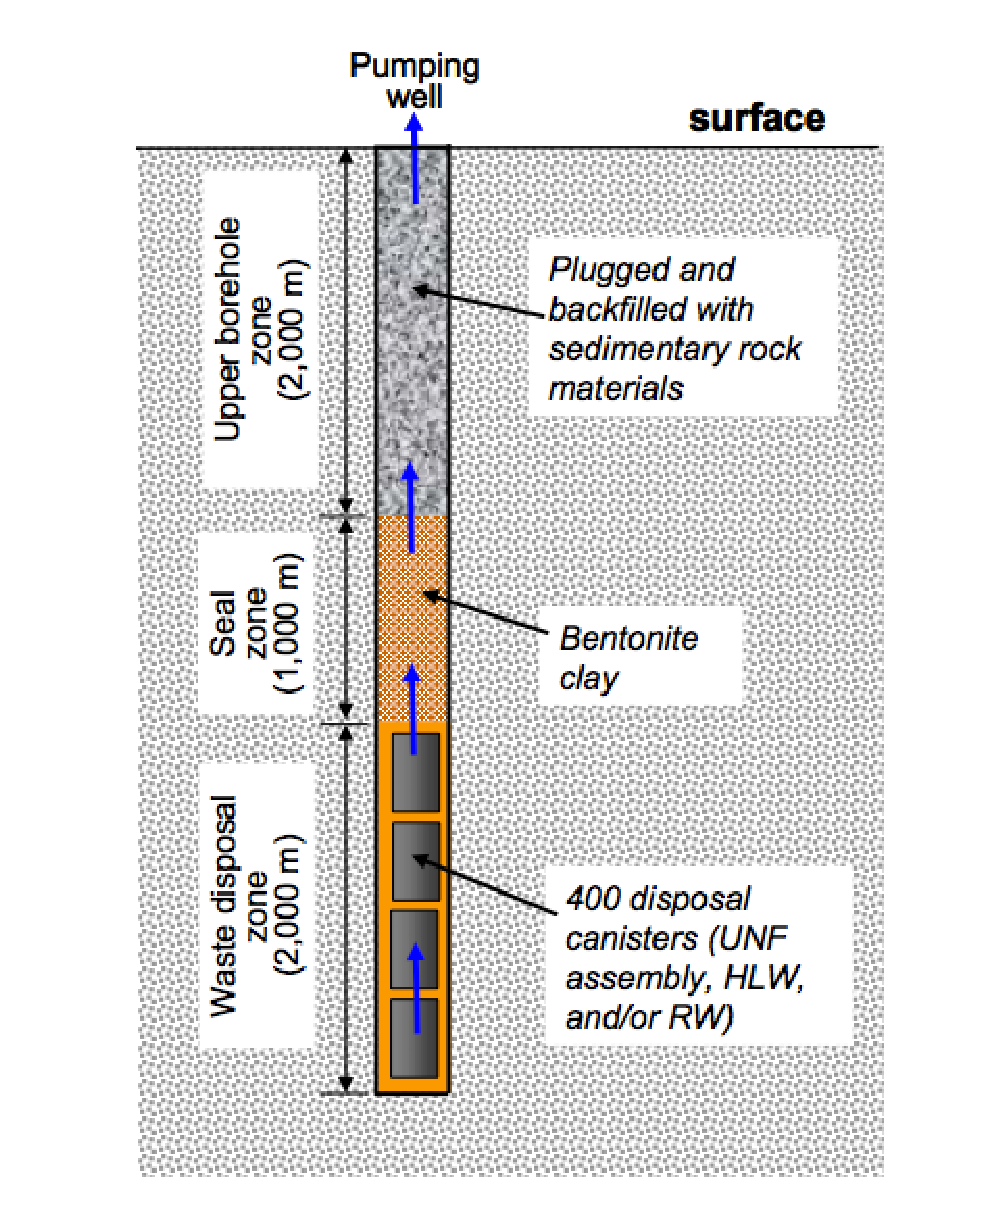
\includegraphics[height=.7\textheight]{./images/boreholeGPAM.eps}
    \end{center}
    \caption{DOE-NE Used Fuel Disposition Campaign Deep Borehole concept 
    \cite{clayton_generic_2011}.}
    \label{fig:boreholeGPAM}
  \end{figure}

\end{frame}


\begin{frame}
  \frametitle{Repository Layouts}

  \begin{minipage}{0.49\textwidth}
    \begin{figure}[h!]
      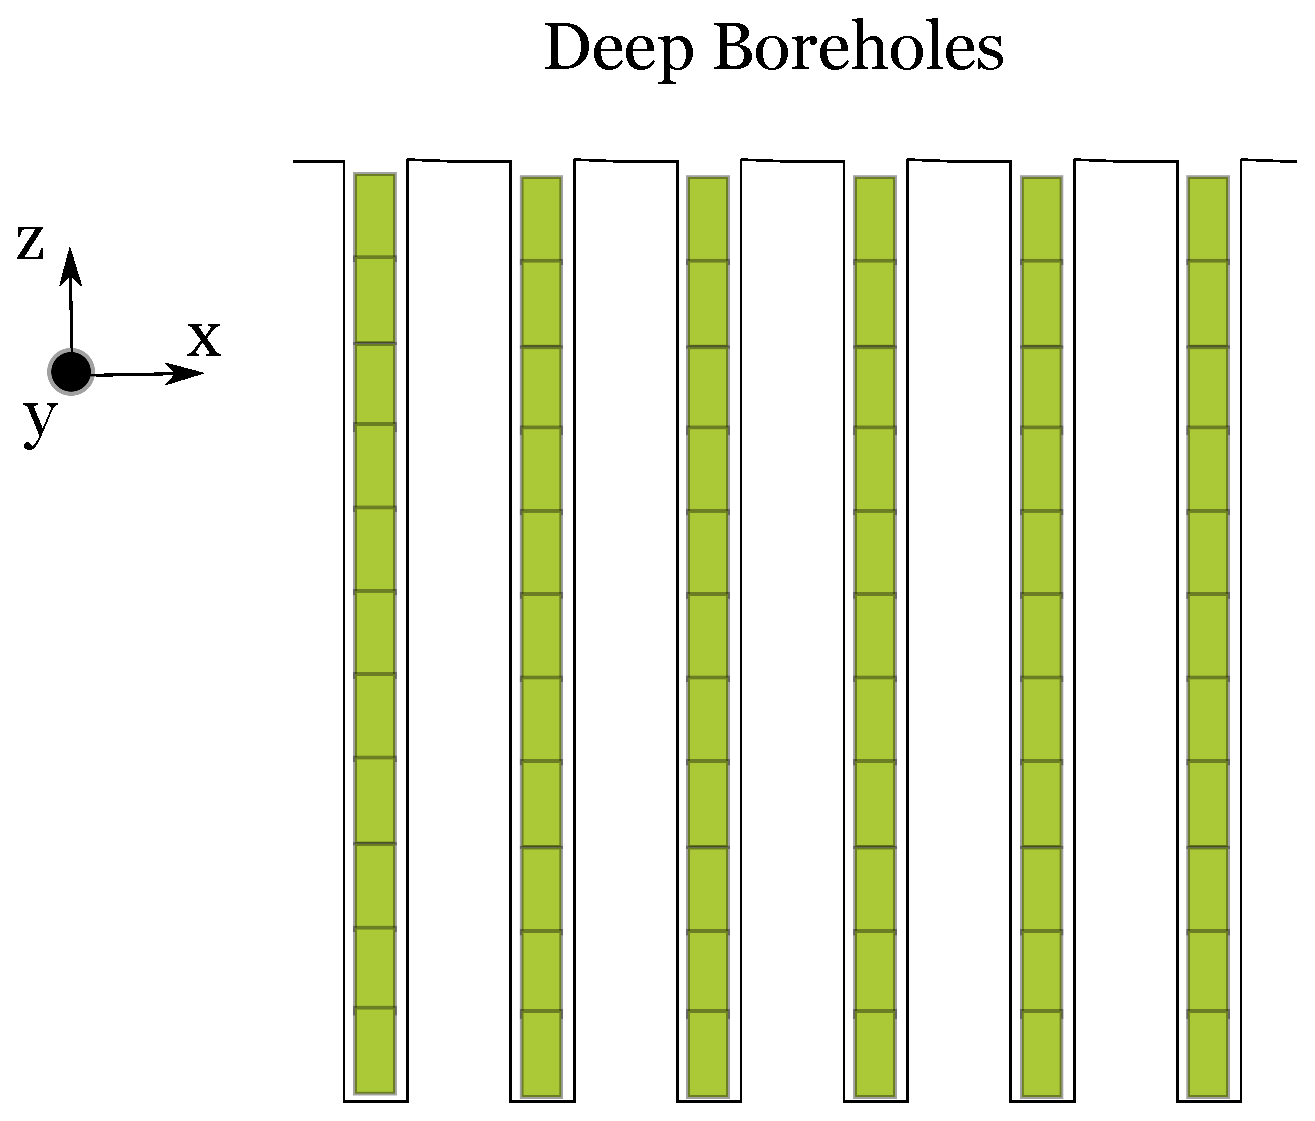
\includegraphics[width=0.75\textwidth]{./images/boreholes.eps}
    \end{figure}
    \begin{figure}[h!]
      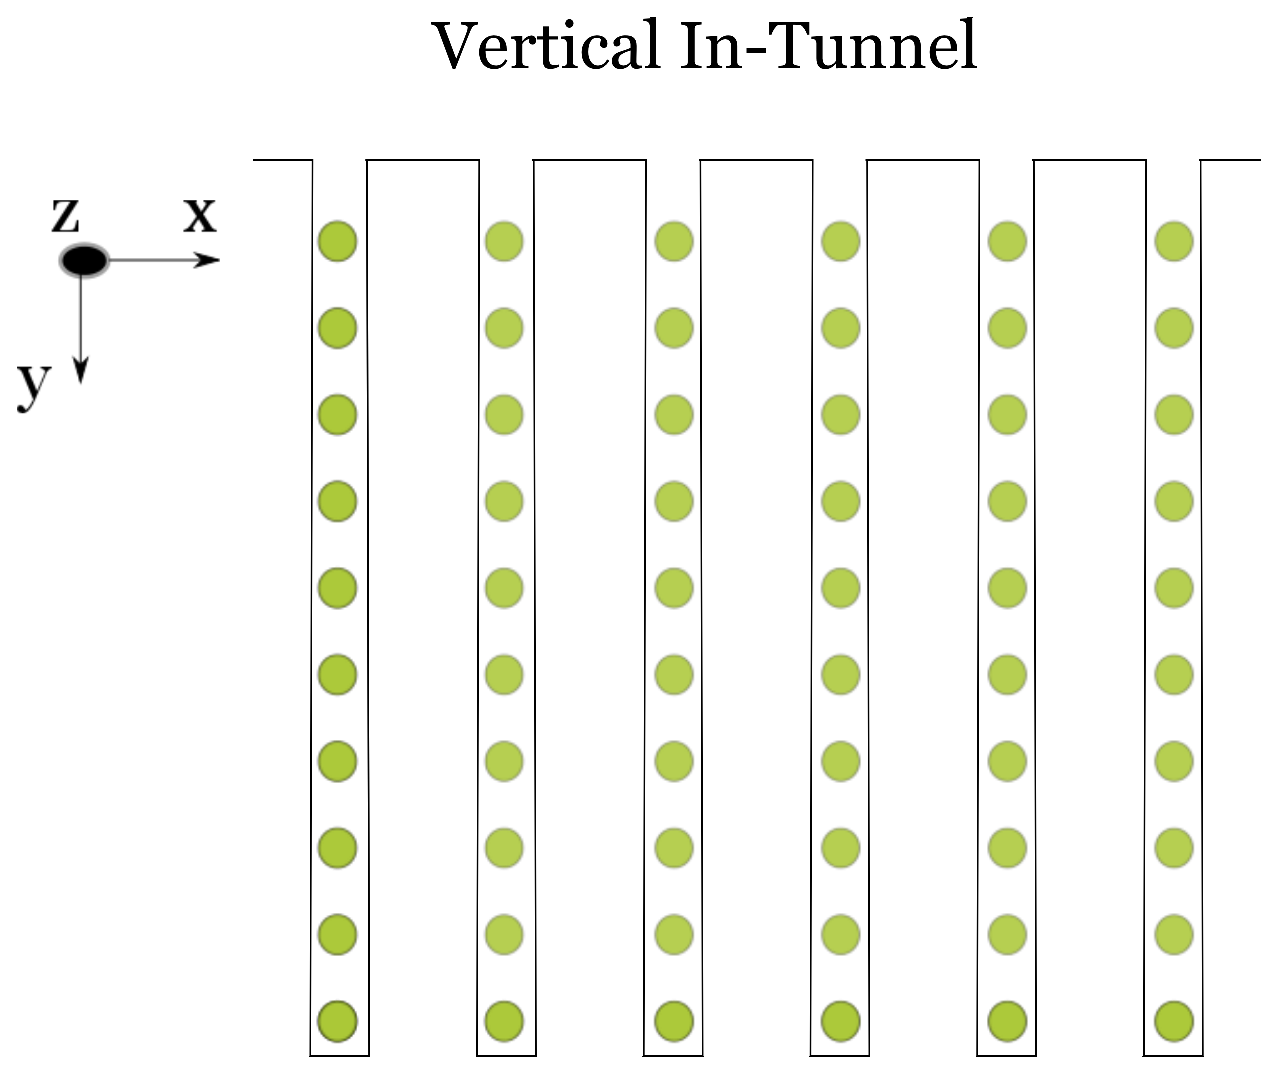
\includegraphics[width=0.75\textwidth]{./images/vertical.eps}
    \end{figure}
  \end{minipage}
  \hspace{0.01cm}
  \begin{minipage}{0.49\textwidth}
    \begin{figure}[h!]
      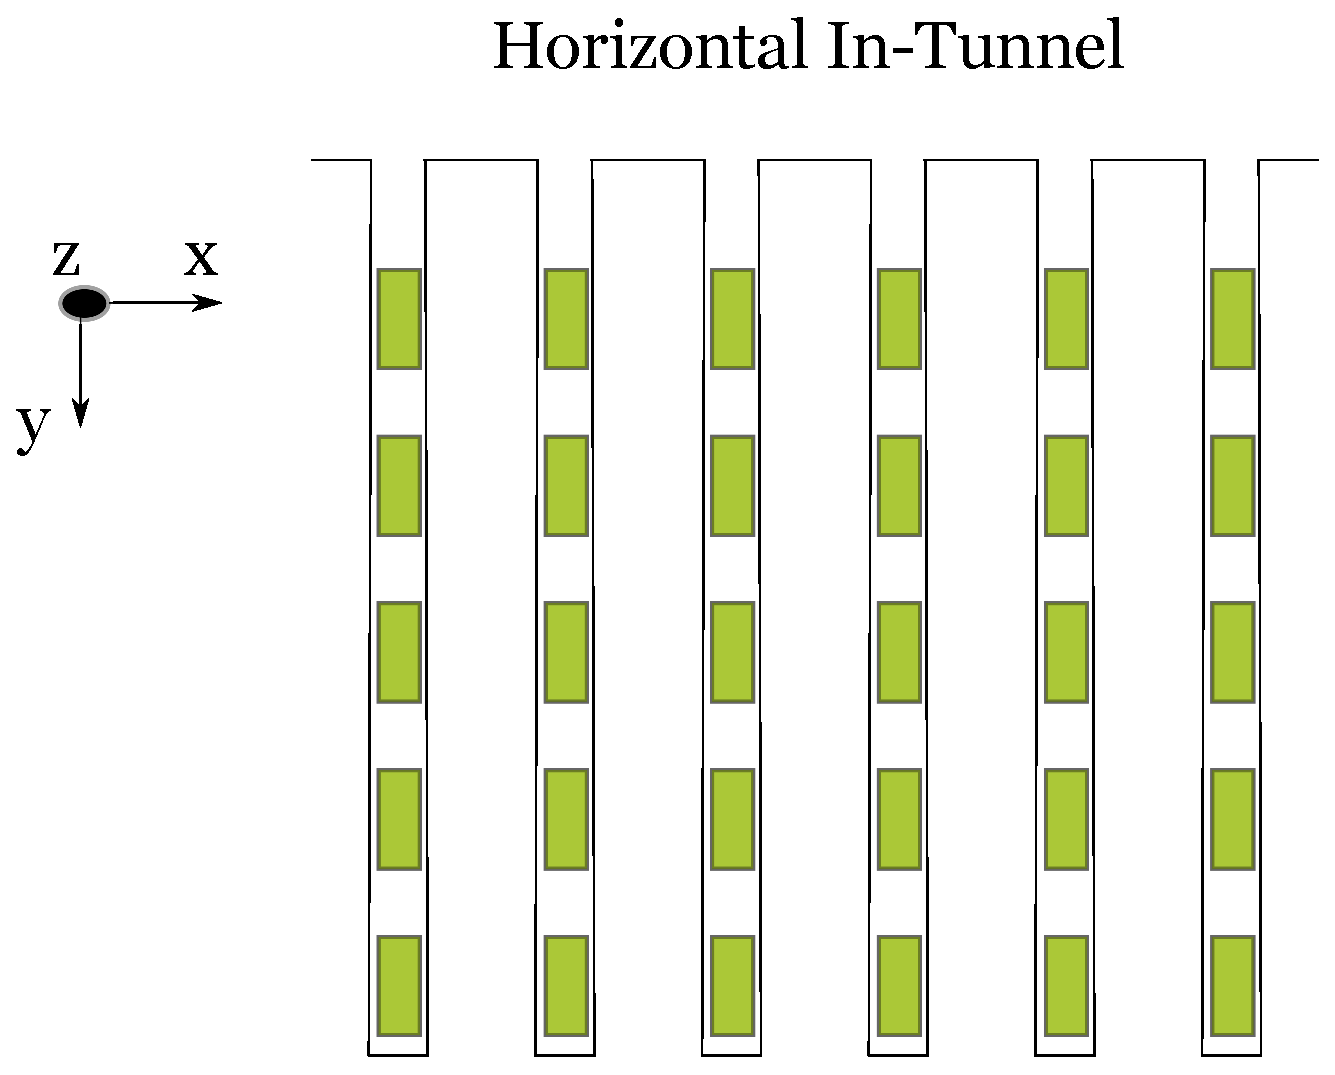
\includegraphics[width=0.8\textwidth]{./images/horizontal.eps}
    \end{figure}
    \begin{figure}[h!]
      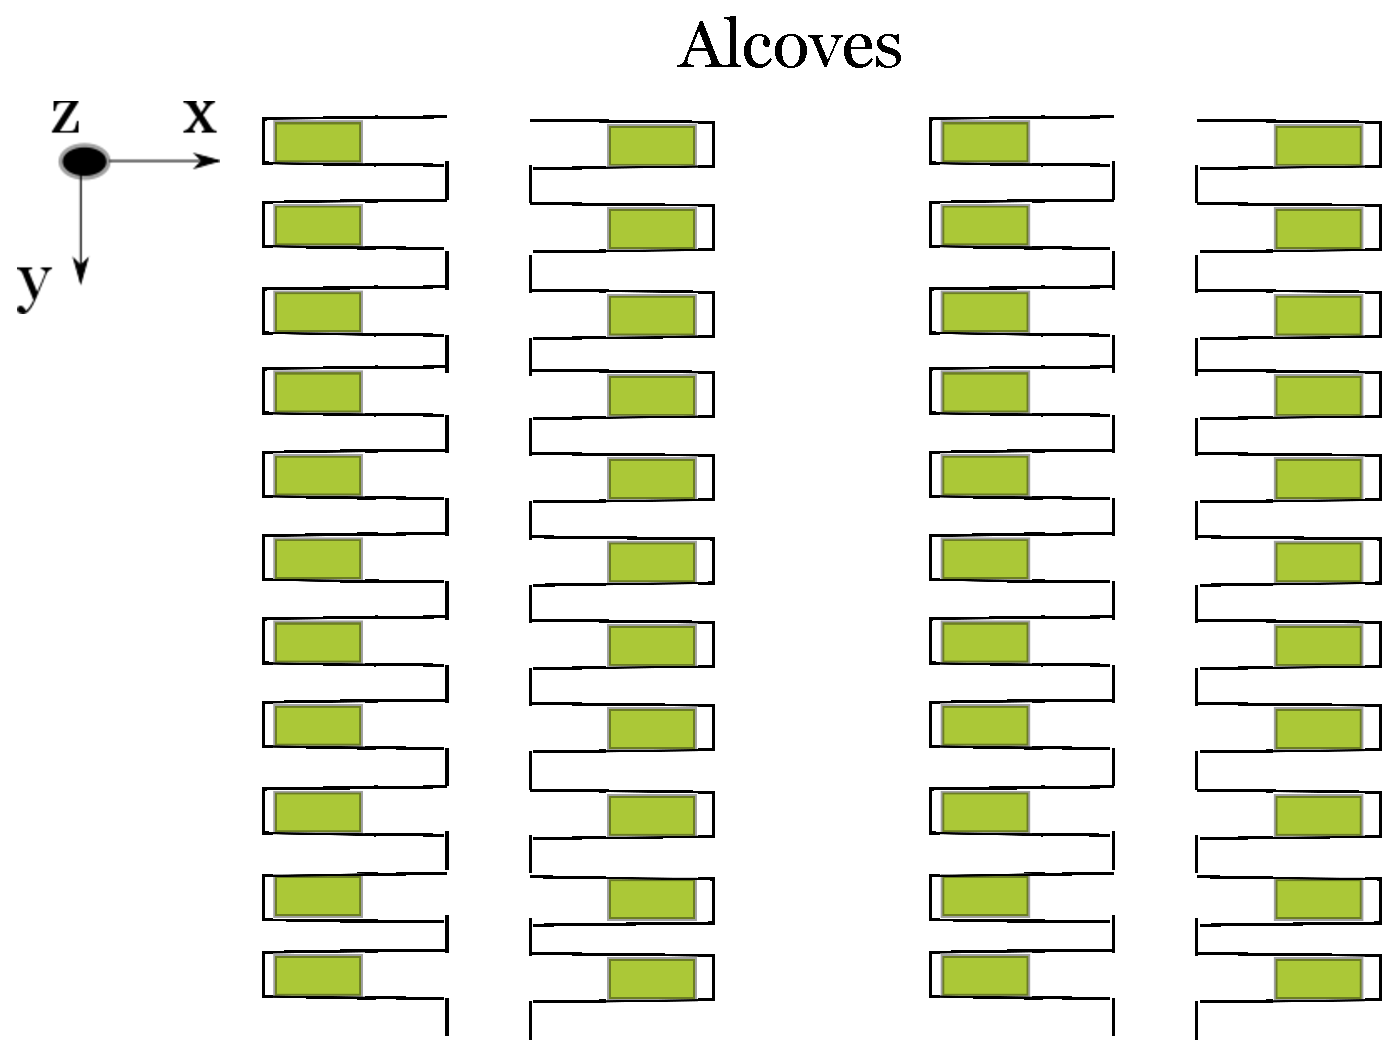
\includegraphics[width=0.8\textwidth]{./images/alcoves.eps}
    \end{figure}
  \end{minipage}

\end{frame}

\begin{frame}[c]
  \frametitle{All Disposal Environments}
  % Table
  %        File: geos_tab.tex
%     Created: Thu Aug 04 11:00 AM 2011 C
% Last Change: Thu Aug 04 11:00 AM 2011 C
%
\begin{table}[h!]
  \centering
  \footnotesize{
  \begin{tabular}{|l|r|r|r|r|}
    \multicolumn{5}{c}{\textbf{Features of Various Concepts}}\\
    \hline
    Feature & Clay & Granite & Salt & Deep Borehole \\ 
    \hline
    \multicolumn{5}{|c|}{\textbf{Hydrology}}\\
    \hline
    Total Porosity $[\%]$    & 34-60  & 0.1 & 0.5 & 0-0.5 \\ 
    Eff. Porosity $[\%]$ & 0.5-5 & 0.0005 & 0.1 & 0.00005-0.01 \\ 
    Conductivity$[m/s]$ & $10^{-11} - 10^{-9}$ & 
    $10^{-6}-10^{-5}$ & $10^{-12}-10^{-10}$ & 
    $10^{-13}-10^{-4}$ \\ 
    Fracturation & none & high & none & low at depth \\ 
    \hline
    \hline
    \multicolumn{5}{|c|}{\textbf{Geochemistry}}\\
    \hline
    Reducing & Near \& Far Field & NF only  & NF only & NF only \\
    Oxidizing & none & Slight in FF & Slight in FF & Slight in FF \\
    Salinity & higher at depth & higher at depth & high & high \\
    pH & $\sim7$ & $\ge7$ & $\ge7$ & $\sim7$ \\
    \hline
    \hline
    \multicolumn{5}{|c|}{\textbf{Design}}\\
    \hline
    Waste Package & Steel, Cu & Steel, Cu & Steel & Steel,Cement \\
    Buffer & -,Fo-Ca,Cement & Fo-Ca,Cement & Crushed Salt & -,Fo-Ca,Cement\\ 
    Depth & 100-500 m & 100-500 m & 100-500m & 3-5km \\ 
    Emplacement & Vert.,Horiz,Alcove & Vert.,Horiz. & Alcove & Vert. \\ 
    Packages/Gallery & one, many & one, many & one, two & 400 \\ 
    \hline
    \hline
    \multicolumn{5}{|c|}{\textbf{Thermal Behavior}}\\
    \hline
    Buffer Limit $[^{\circ}C]$ & 100 (Fo-Ca) & 100 (Fo-Ca) & 180 & 100 (Fo-Ca) \\ 
    Host Limit $[^{\circ}C]$   & 100 (alteration)  & 200 (cracking) & 180 (brines) & none \\ 
    Conductivity $[\frac{W}{m{\cdot}K}]$ & $1-2$ & $2-4$ & $\sim4$  & $2-4$ \\ 
    Coalesence & yes & no & yes & no \\ 
    \hline
  \end{tabular}
  }
  \label{tab:geos_tab}
\end{table}
%  \cite{stober_hydraulic_2006} 

\end{frame}




%%----------------------------------------%%
\begin{frame}
  \frametitle{Repository Components}
\footnotesize{
  \begin{figure}[htbp!]
  \begin{center}
    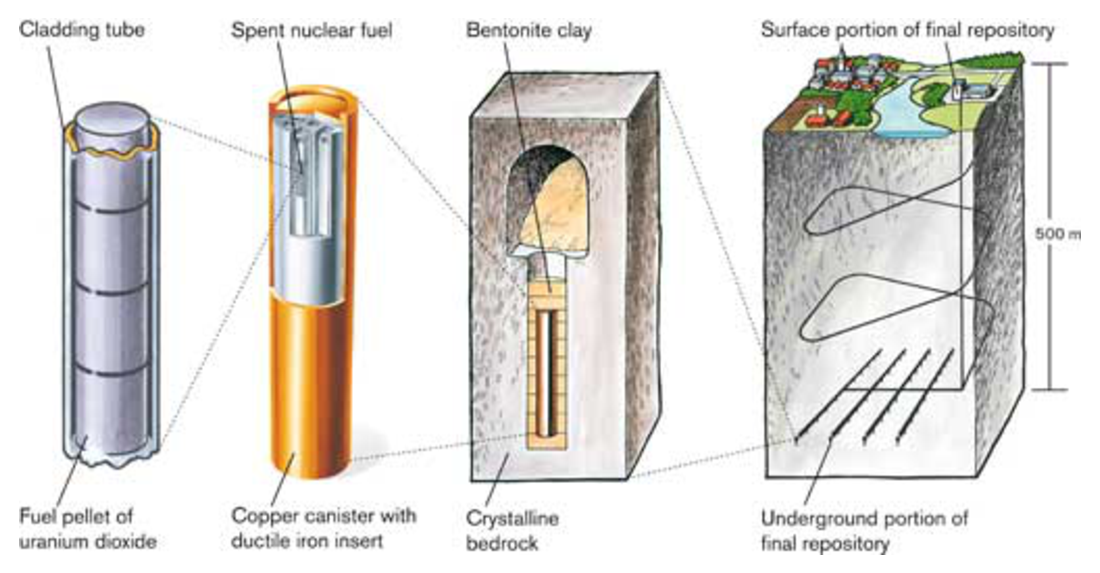
\includegraphics[width=0.7\textwidth]{./images/skb_components.eps}
  \end{center}
  \caption{Geologic disposal systems typically employ engineered barrier 
    systems as well as natural barrier systems. This is a Swedish concept in 
    granite \cite{ab_long-term_2006}.}
  \label{fig:skb_components}
\end{figure}

}
\end{frame}


\begin{frame}
  \frametitle{Repository Layouts}

  \begin{minipage}{0.49\textwidth}
    \begin{figure}[h!]
      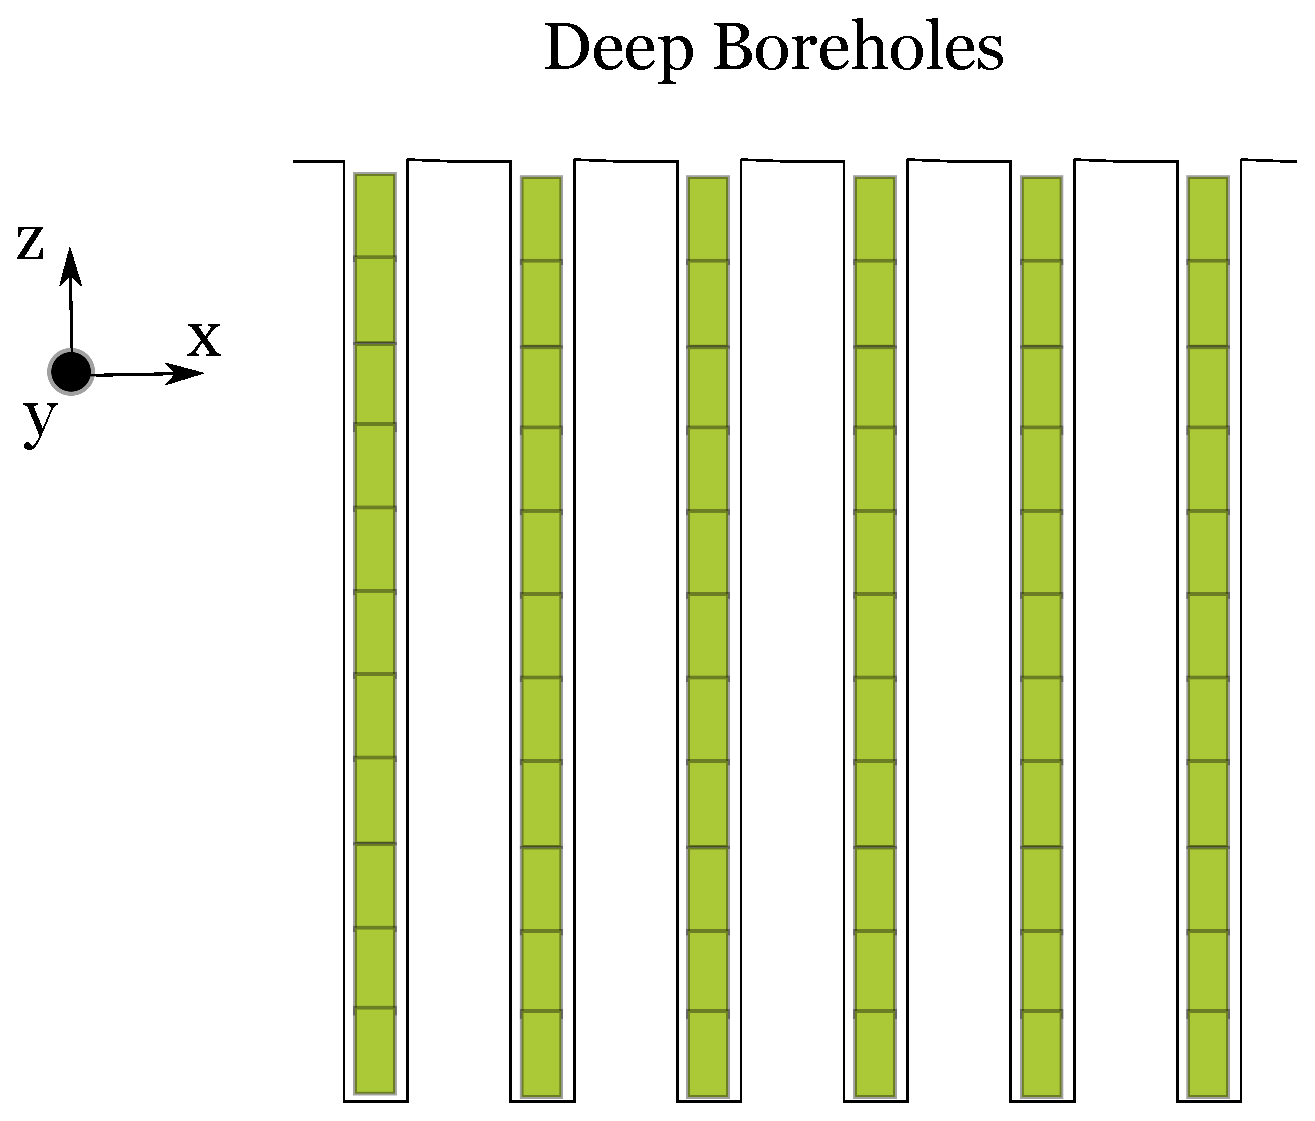
\includegraphics[width=0.75\textwidth]{./images/boreholes.eps}
    \end{figure}
    \begin{figure}[h!]
      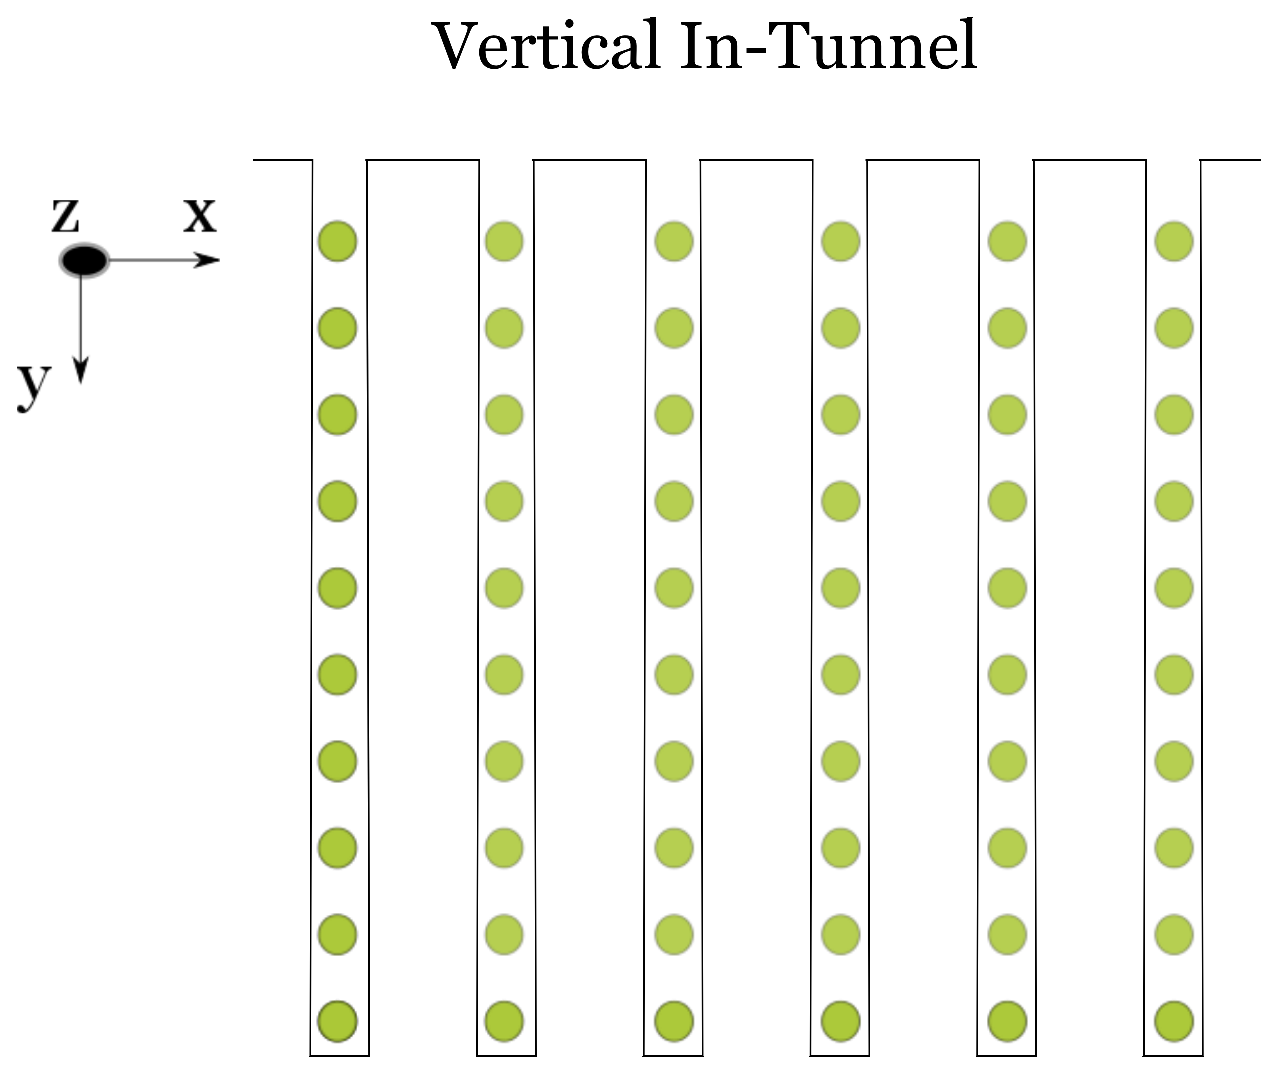
\includegraphics[width=0.75\textwidth]{./images/vertical.eps}
    \end{figure}
  \end{minipage}
  \hspace{0.01cm}
  \begin{minipage}{0.49\textwidth}
    \begin{figure}[h!]
      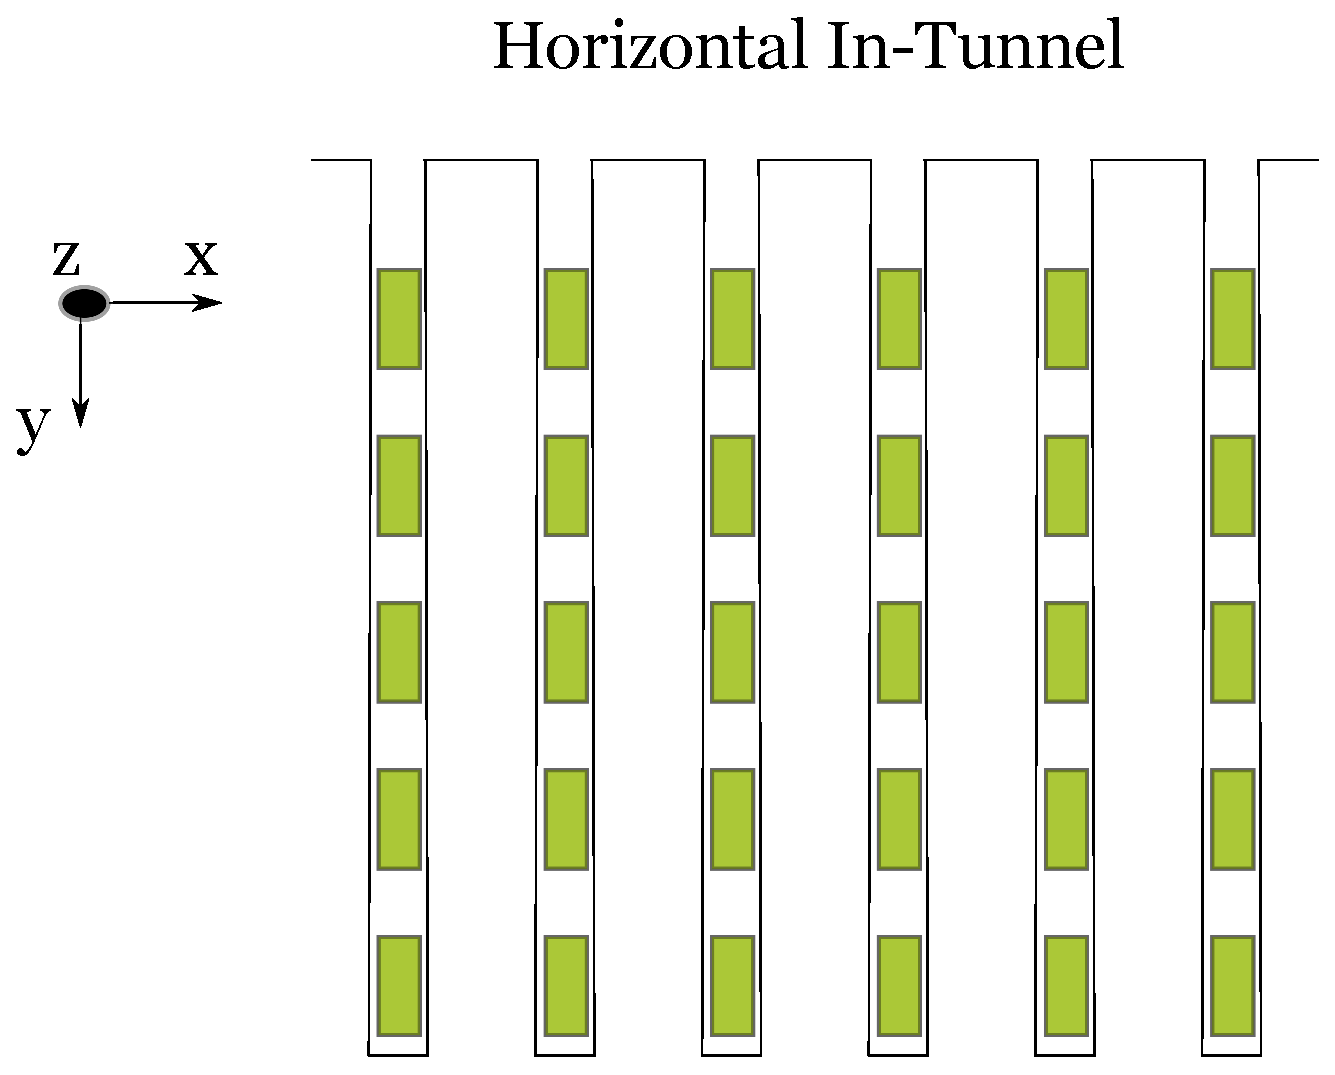
\includegraphics[width=0.8\textwidth]{./images/horizontal.eps}
    \end{figure}
    \begin{figure}[h!]
      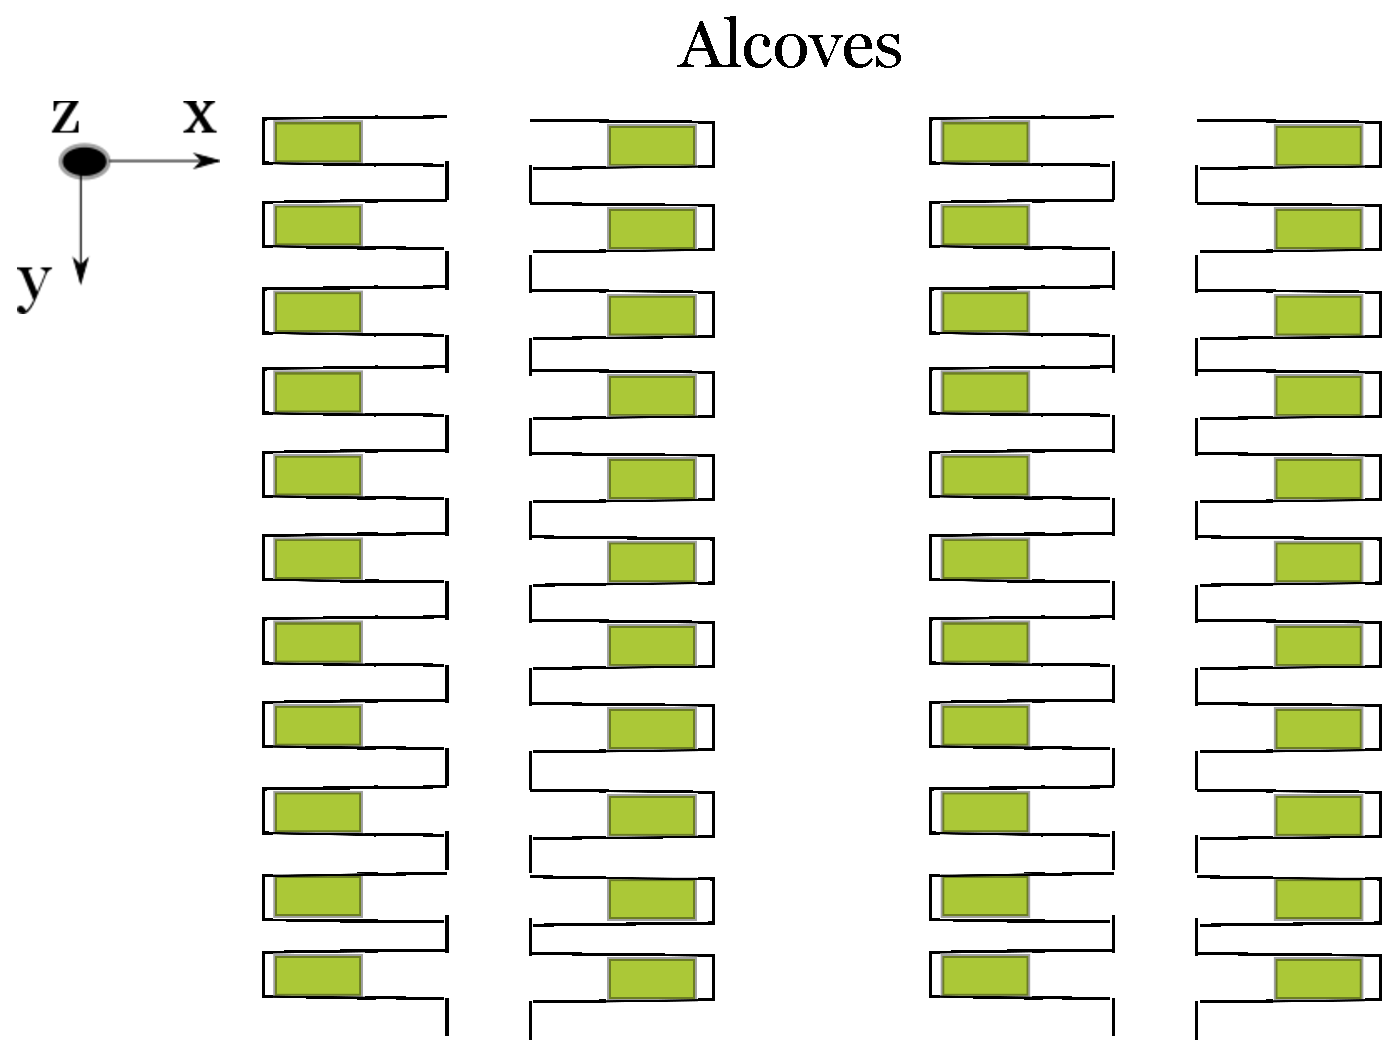
\includegraphics[width=0.8\textwidth]{./images/alcoves.eps}
    \end{figure}
  \end{minipage}

\end{frame}

\begin{frame}
  \footnotesize{
  \frametitle{Unsaturated, Ventilated Concepts}
  \begin{figure}[htbp!]
  \begin{center}
    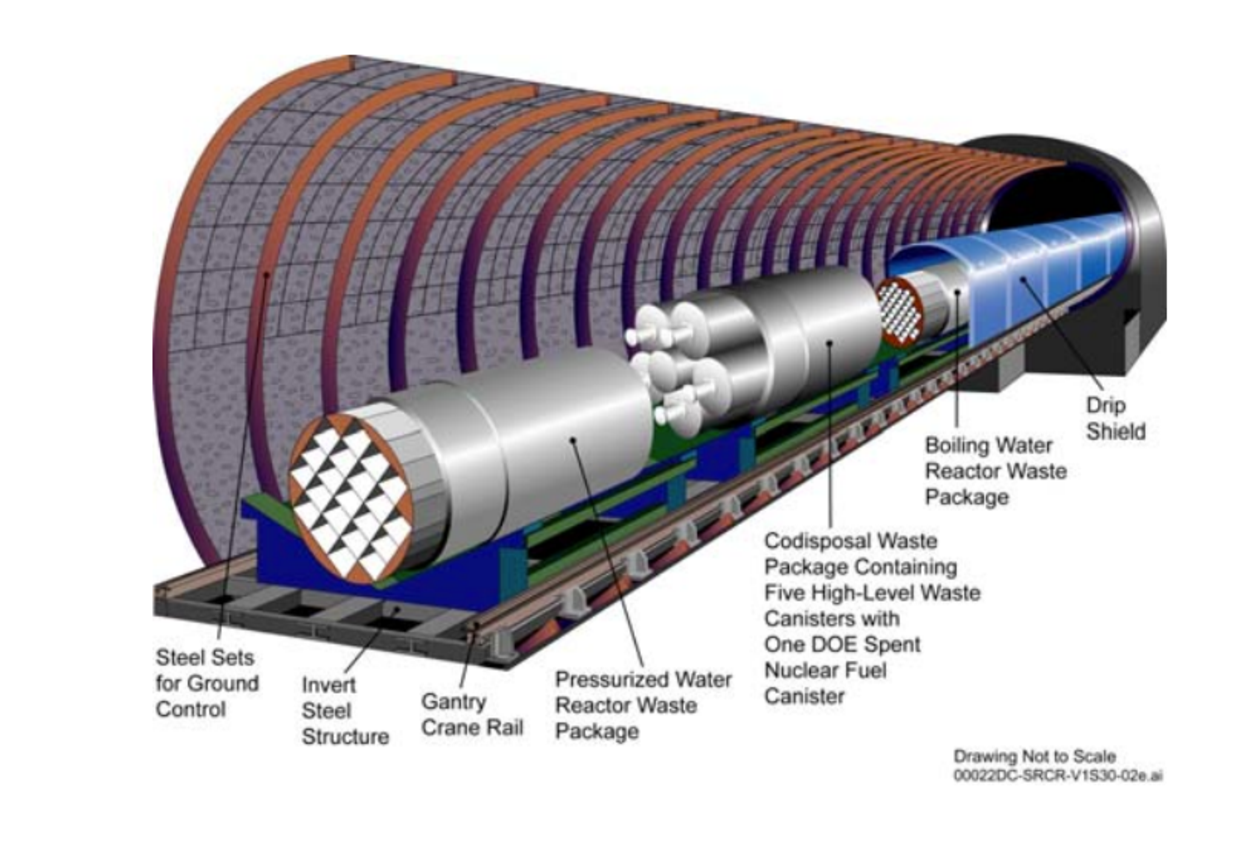
\includegraphics[height=0.7\textwidth]{./images/yucca_tunnel.eps}
  \end{center}
  \caption{The current U.S. geologic disposal concept \cite{peters_whats_2013}.}
  \label{fig:yucca_tunnel}
\end{figure}

}
\end{frame}

\begin{frame}
  \footnotesize{
  \frametitle{Saturated , Enclosed Concepts} 
 \begin{figure}[h!]
    \begin{center}
      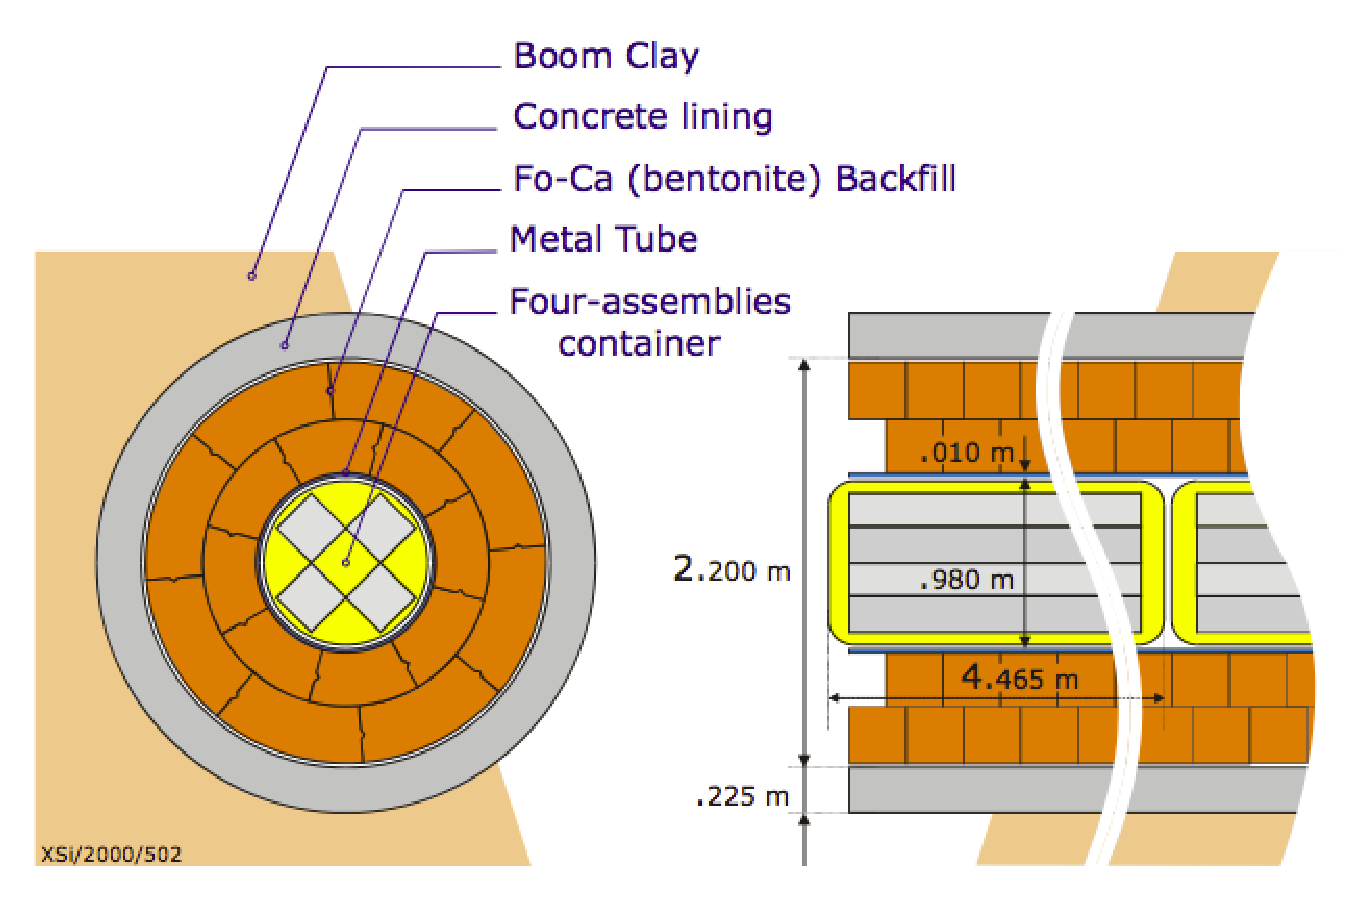
\includegraphics[height=.7\textheight]{./images/belgianClayRedImp.eps}
    \end{center}
    \caption{The Belgian reference concept in Boom Clay is backfilled very soon
   after waste emplacement without a ventilation period and is located below the water table
   \cite{von_lensa_red-impact_2008}.}
    \label{fig:belgianClayRedImp}
  \end{figure}
}
\end{frame}



\begin{frame}
  \frametitle{Tuff (Yucca) Disposal Environments}
  \footnotesize{
    \begin{figure}[htbp!]
  \begin{center}
    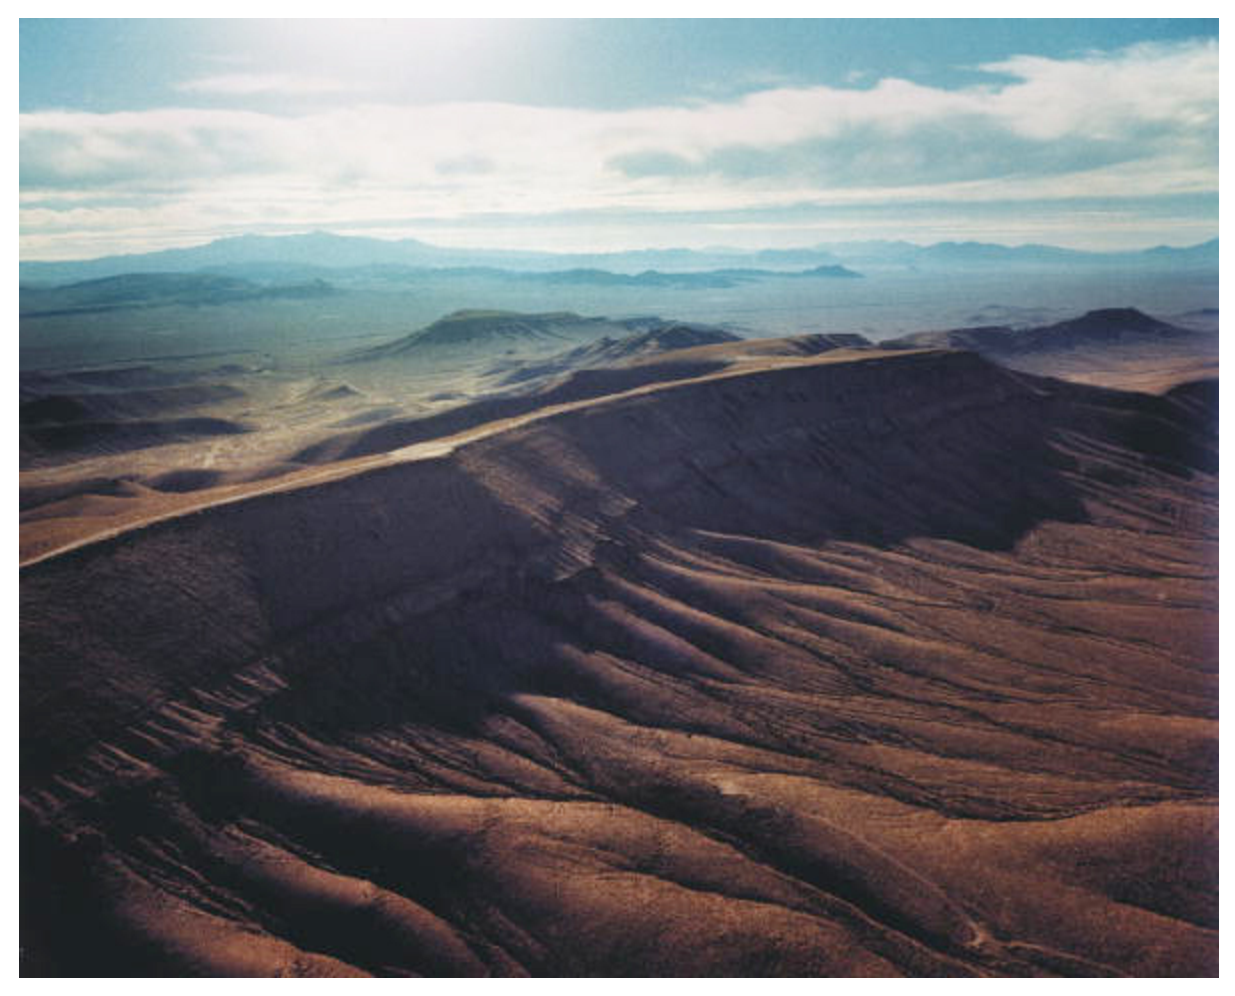
\includegraphics[width=0.5\textwidth]{./images/yucca_site.eps}
  \end{center}
  \caption{Yucca Mountain is in southern Nevada \cite{omb_yucca_2006}.}
  \label{fig:yucca_site}
\end{figure}

  }
\end{frame}

\begin{frame}
  \frametitle{Alternative Disposal Geology Options}
   \begin{minipage}{0.44\textwidth}
     \begin{figure}[h!]
         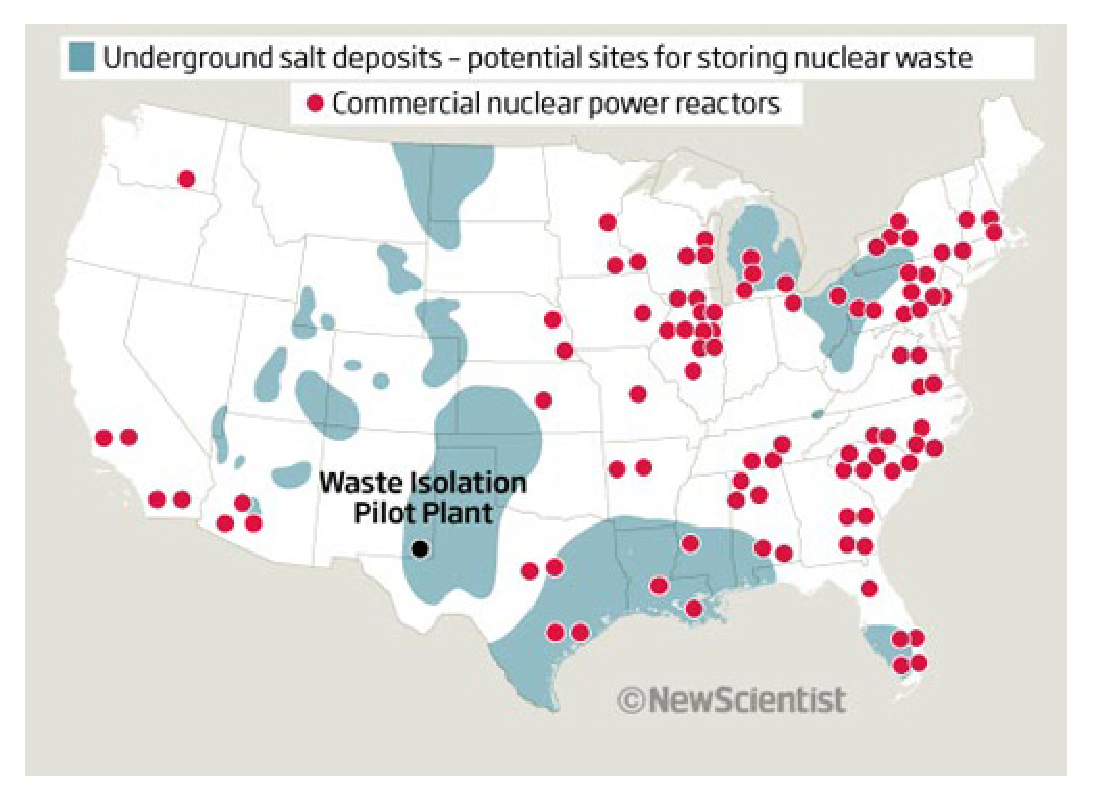
\includegraphics[width=0.8\textwidth]{./images/saltNewScientist.eps}
         \caption{U.S. Salt Deposits, ref. \cite{newscientist_where_2011}.}
     \end{figure}
     \begin{figure}[h!]
         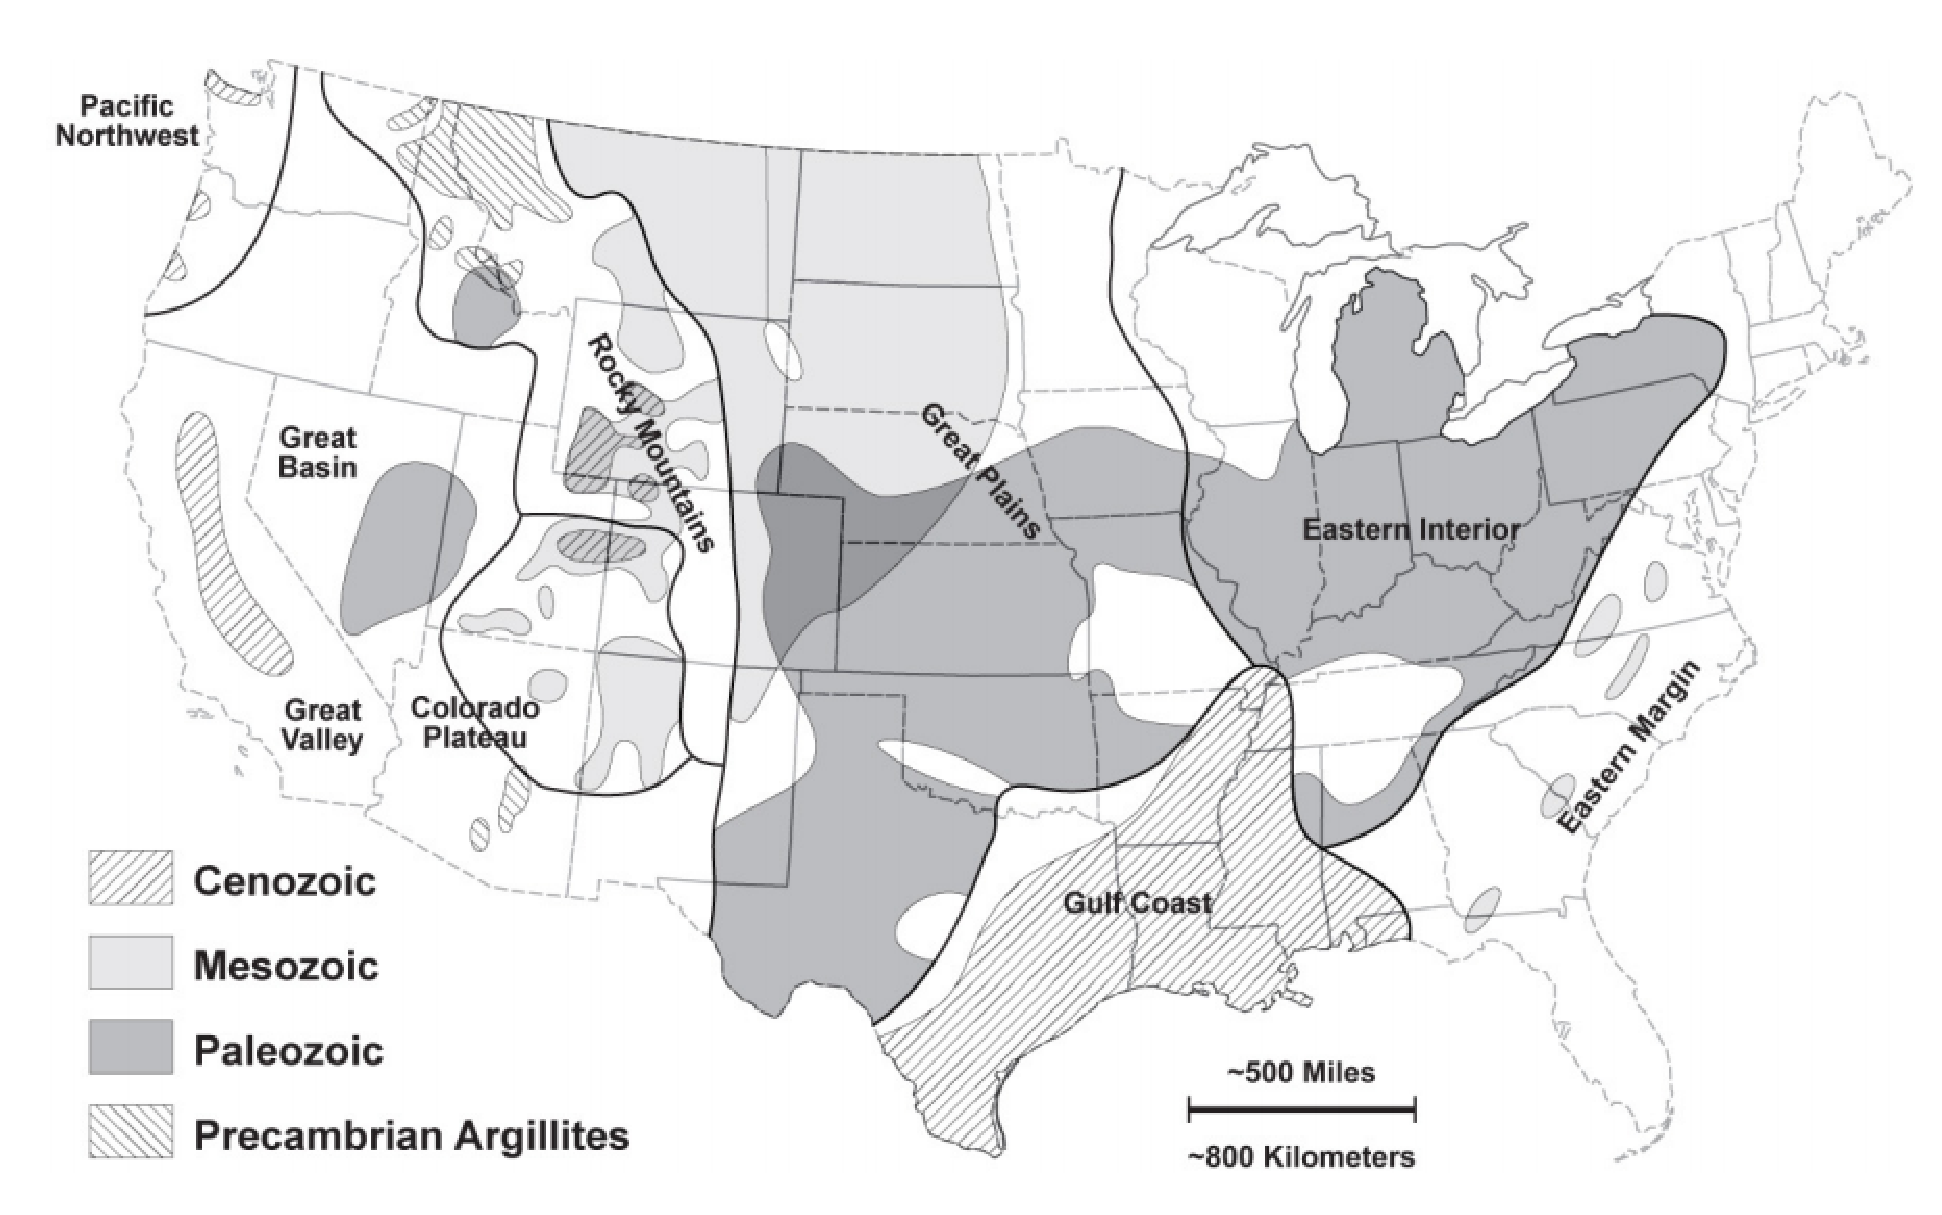
\includegraphics[width=0.8\textwidth]{./images/clayGonzales.eps}
         \caption{U.S. Clay Deposits, ref. \cite{gonzales_shales_1985}.}
     \end{figure}
   \end{minipage}
   \hspace{0.01cm}
   \begin{minipage}{0.44\textwidth}
     \begin{figure}[h!]
         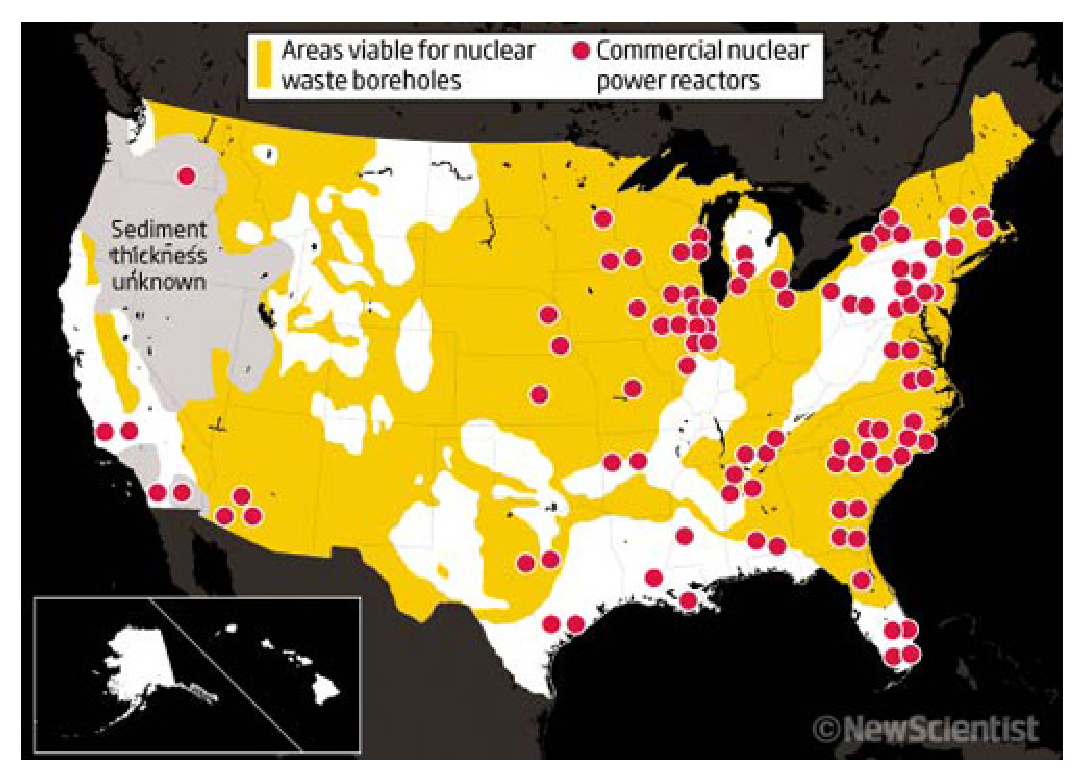
\includegraphics[width=0.8\textwidth]{./images/boreholeNewScientist.eps}
         \caption{U.S. Crystalline Basement, ref.  \cite{newscientist_where_2011}.}
     \end{figure}
     \begin{figure}[h!]
         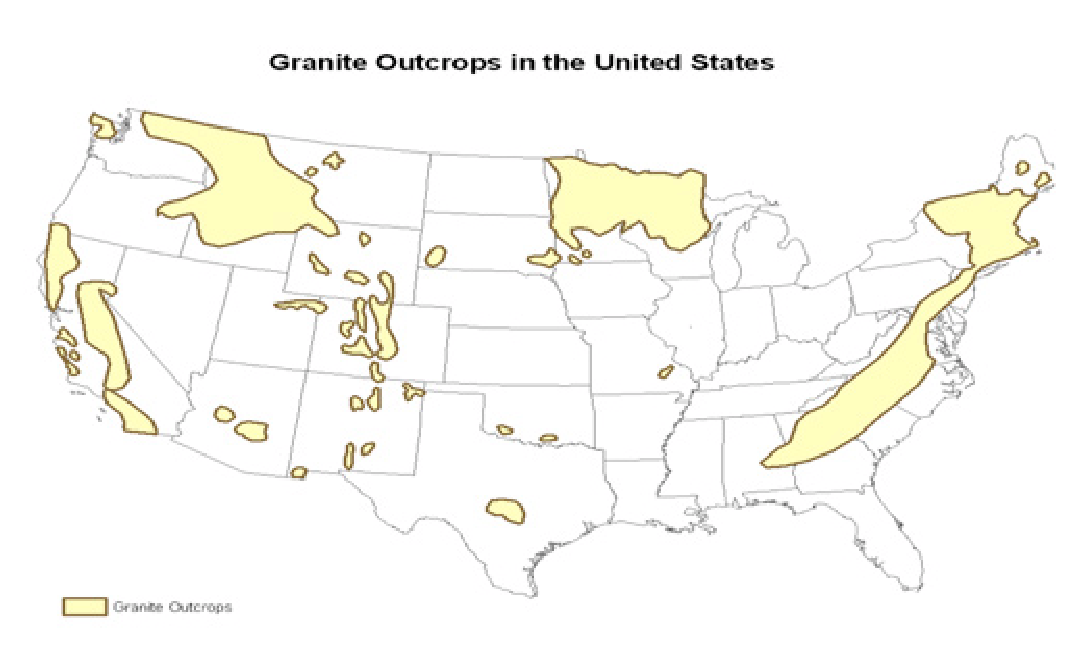
\includegraphics[width=0.8\textwidth]{./images/graniteBush.eps}
         \caption{U.S. Granite Beds, ref. \cite{bush_economic_1976}.}
     \end{figure}
   \end{minipage}
\end{frame}

\begin{frame}
  \frametitle{Clay Disposal Environments}
  \footnotesize{

  \begin{figure}[h!]
    \begin{center}
      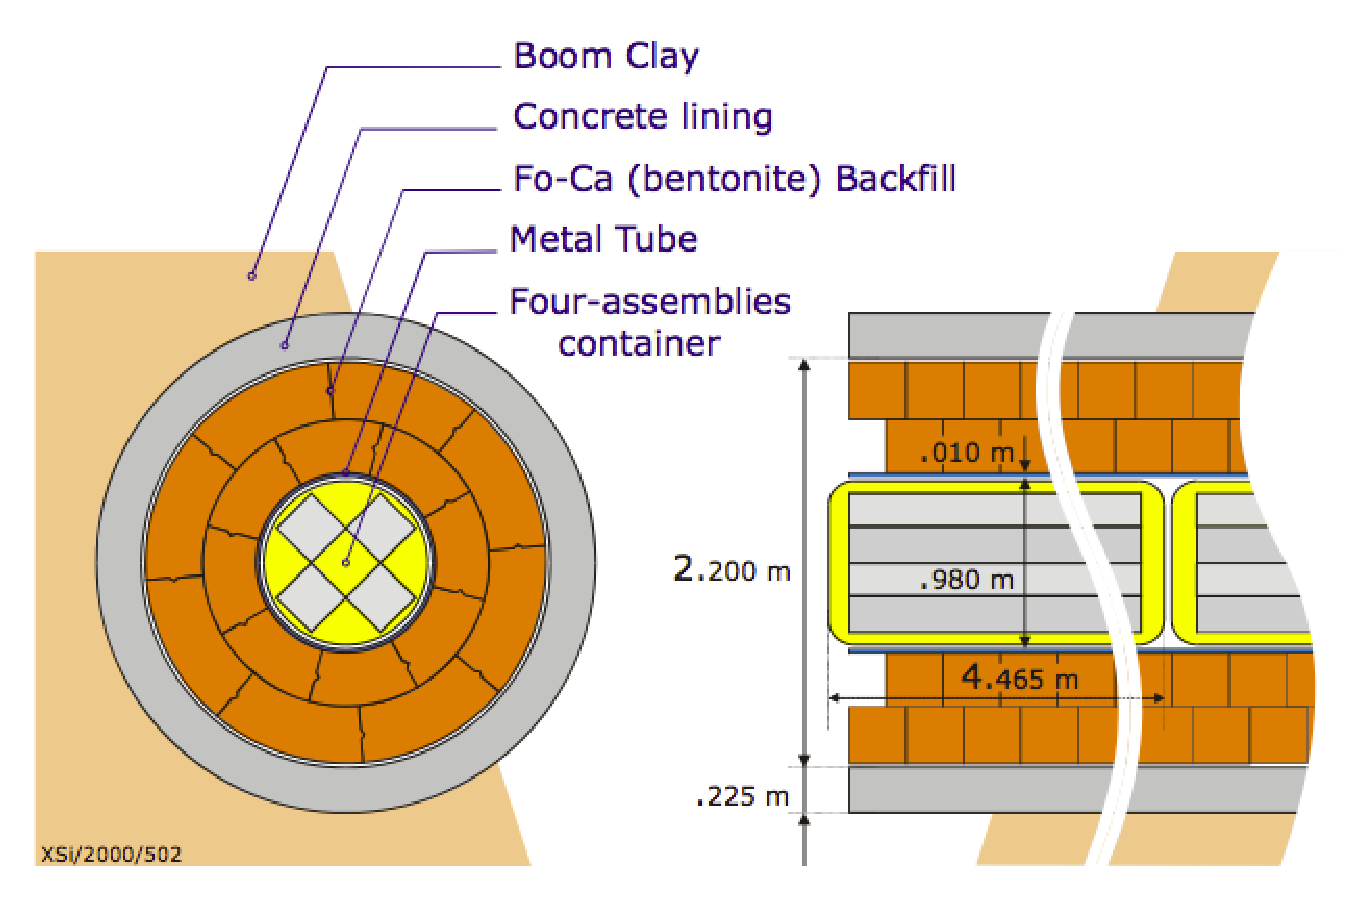
\includegraphics[height=.7\textheight]{./images/belgianClayRedImp.eps}
    \end{center}
    \caption{Belgian reference concept in Boom Clay 
    \cite{von_lensa_red-impact_2008}.}
    \label{fig:belgianClayRedImp}
  \end{figure}

}
\end{frame}

\begin{frame}
  \frametitle{Granite Disposal Environments}
  \footnotesize{

  \begin{figure}[h!]
    \begin{center}
      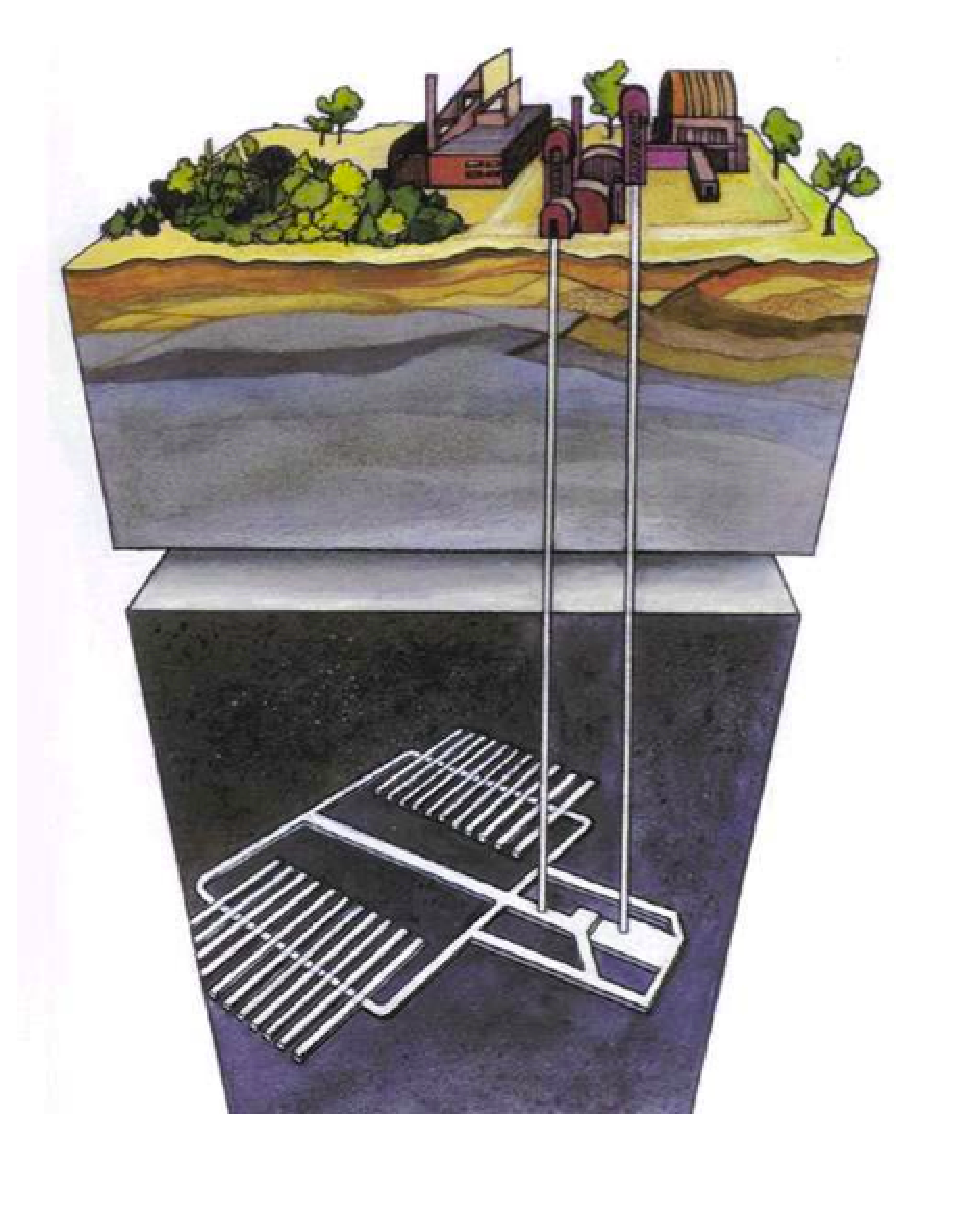
\includegraphics[height=.7\textheight]{./images/czechGraniteRedImp.eps}
    \end{center}
    \caption{Czech reference concept in Granite 
    \cite{von_lensa_red-impact_2008}.}
    \label{fig:czechGraniteRedImp}
  \end{figure}
}
\end{frame}

\begin{frame}
  \frametitle{Salt Disposal Environments}
  \footnotesize{

  \begin{figure}[h!]
    \begin{center}
      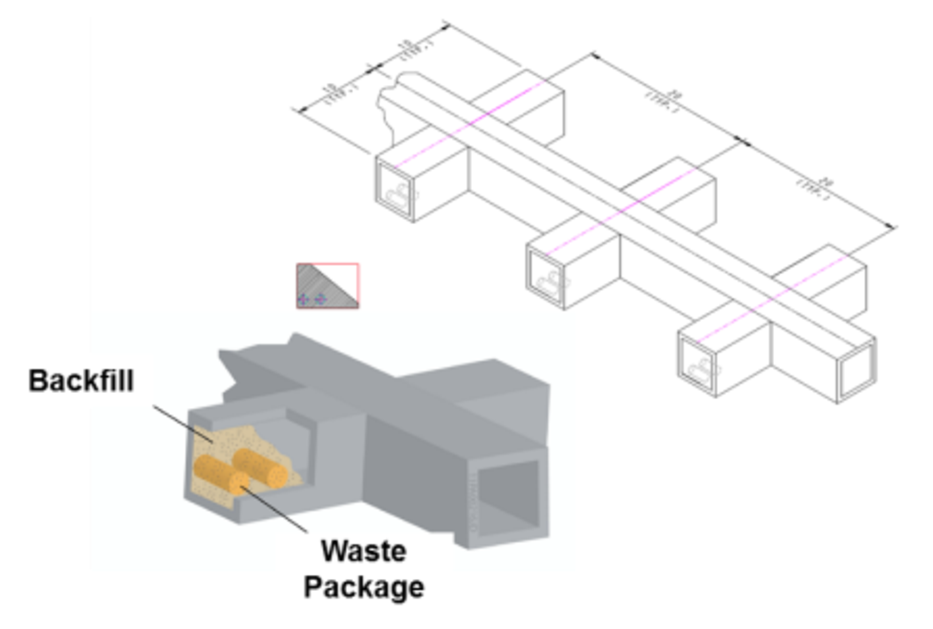
\includegraphics[height=.7\textheight]{./images/carter_salt_layout.eps}
    \end{center}
    \caption{DOE-NE Used Fuel Disposition Campaign  concept in 
    Salt \cite{hardin_generic_2011}.}
    \label{fig:salt_layout}
  \end{figure}
}
\end{frame}
\begin{frame}
  \frametitle{Salt Disposal Environments}
  \footnotesize{

  \begin{figure}[h!]
    \begin{center}
      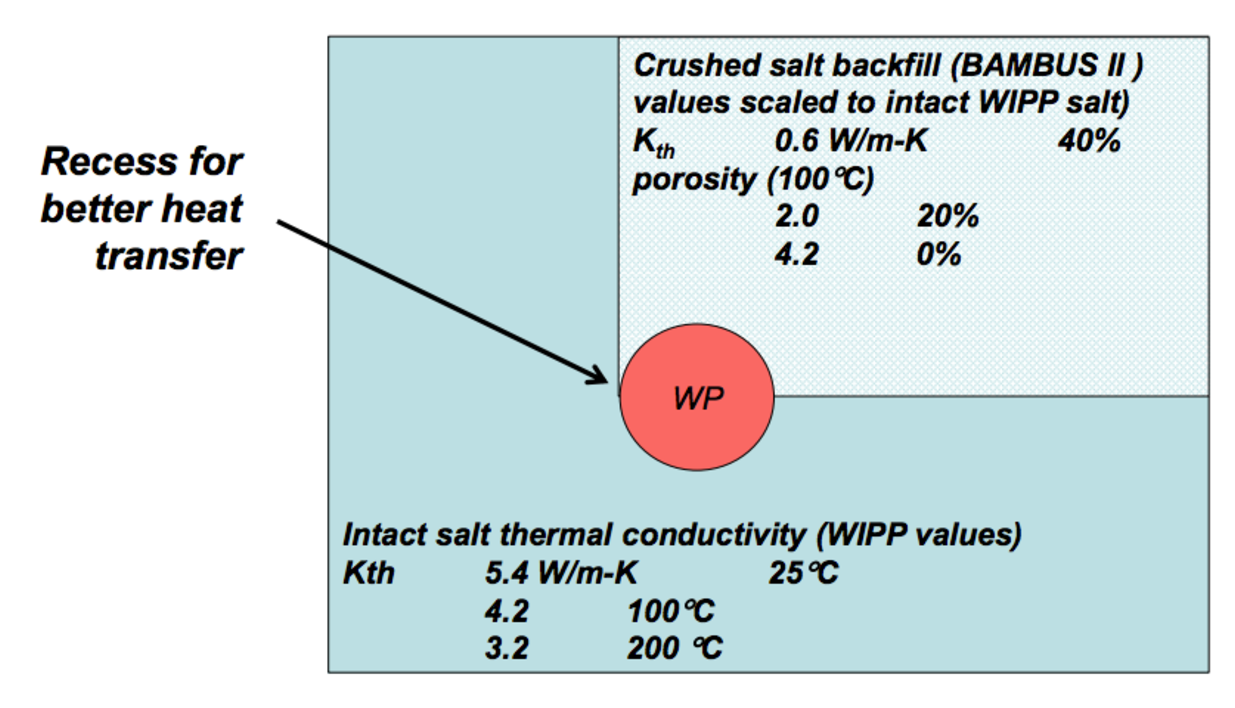
\includegraphics[height=.7\textheight]{./images/hardin_salt_layout.eps}
    \end{center}
    \caption{DOE-NE Used Fuel Disposition Campaign  concept in 
    Salt \cite{hardin_generic_2011}.}
    \label{fig:hardin_salt_layout}
  \end{figure}
}
\end{frame}

\begin{frame}
  \frametitle{Deep Borehole Disposal Environment}
  \footnotesize{

  \begin{figure}[h!]
    \begin{center}
      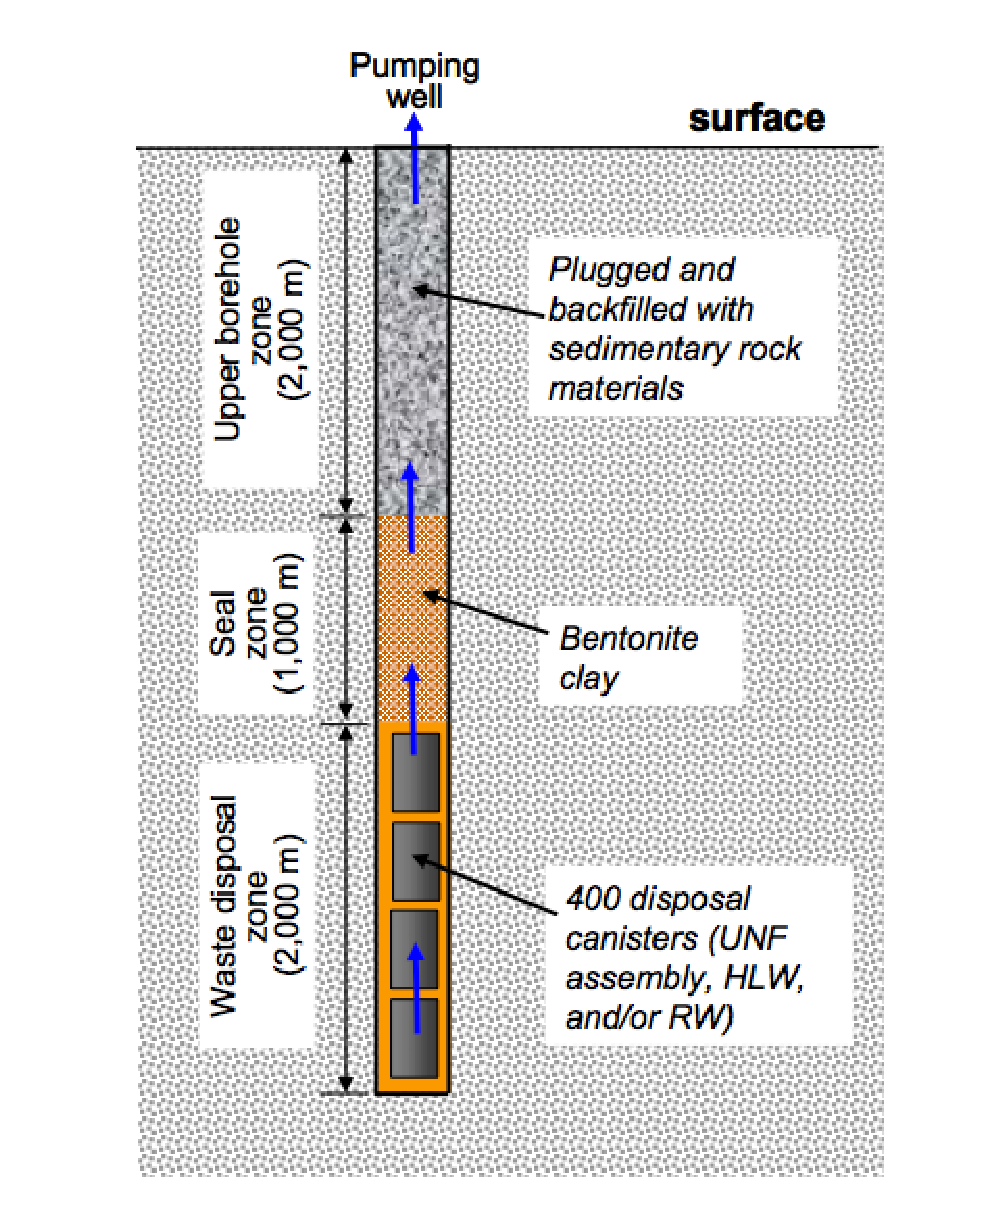
\includegraphics[height=.7\textheight]{./images/boreholeGPAM.eps}
    \end{center}
    \caption{DOE-NE Used Fuel Disposition Campaign Deep Borehole concept 
    \cite{hardin_generic_2011}.}
    \label{fig:boreholeGPAM}
  \end{figure}
}
\end{frame}



%%--------------------------------%%
%%--------------------------------%%
\begin{frame}[allowframebreaks]
  \frametitle{References}
  \bibliographystyle{plain}
  {\footnotesize \bibliography{bibliography} }

\end{frame}

%%--------------------------------%%


\end{document}



